\documentclass[a4paper,12pt,titlepage]{report}

\usepackage[spanish,activeacute]{babel}
\usepackage[fixlanguage]{babelbib}
\usepackage{graphicx}
\usepackage{amssymb}
\usepackage{ifthen}
%\usepackage{fancyhdr}
\usepackage{fullpage}
\usepackage{tabularx}
\usepackage{subfigure}
\usepackage{moreverb}
\usepackage{titleref}
\usepackage{pdfpages}
\usepackage[font=small]{caption}

% Javier
\usepackage{algorithm}
\usepackage{algpseudocode}
\usepackage[utf8x]{inputenc}
\usepackage{amsmath}
\usepackage{url}
\usepackage{longtable}
\usepackage{multirow}

%\usepackage{titlesec}
% Javier

\usepackage[refpages]{gloss}
\makegloss
\renewcommand{\glossname}{Glosario}
\gloss[nocite]{*}

\begin{document}

\renewcommand{\tablename}{Tabla}
\newcommand{\HRule}{\rule{\linewidth}{0.5mm}}
\newcommand{\Keywords}[1]{\par\noindent
{\small{\textbf{Palabras clave}}: #1}}

\pagestyle{empty}

\begin{titlepage}

\begin{center}

% Upper part of the page

\includegraphics[width=0.2\textwidth]{./Portada/logo}\\[1cm]

\textsc{\LARGE Laboratorio de medios, Instituto de Computación, Facultad de Ingeniería, UDELAR.}\\[1.5cm]

\textsc{\Large Informe de Proyecto de Grado}\\[0.5cm]

% Title
\HRule \\[0.4cm]
{ \huge \bfseries Proyección sobre superficies irregulares}\\[0.4cm]

\HRule \\[1.5cm]

% Author and supervisor
\begin{minipage}{0.45\textwidth}
\begin{flushleft} \large
\emph{Estudiantes:}\\
Daniel \textsc{Gomez de Souza}\\
Javier \textsc{Fradiletti}\\
Adriana \textsc{Soucoff}
\end{flushleft}
\end{minipage}
\begin{minipage}{0.45\textwidth}
\begin{flushright} \large
\emph{Tutor:} \\
Tomás \textsc{Laurenzo}
\end{flushright}
\end{minipage}

\vfill

% Bottom of the page
{\large Montevideo, Uruguay, año 2012.}

\end{center}

\end{titlepage} 

\clearpage\mbox{}\clearpage

\newpage

%\titlespacing*{\chapter}{0pt}{-50pt}{20pt}
%\titleformat{\chapter}[display]{\normalfont\huge\bfseries}{\chaptertitlename\ \thechapter}{20pt}{\Huge}

\pagestyle{plain}
\setcounter{page}{1}
\tableofcontents

\chapter{Introducción}%No se menciona 'proyeccion sobre superficies irregulares directamente'%

La proyección de imágenes sobre una superficie plana mediante un foco luminoso es una técnica con variadas aplicaciones, siendo de las más utilizadas la proyección de películas cinematográficas. En los últimos tiempos se introdujeron dispositivos de video que permiten proyectar la salida de una computadora, los cuales son comúnmente utilizados en ámbitos académicos y empresariales con fines de dictado de cursos y presentaciones. En los últimos años se ha ido popularizando la proyección de imágenes y videos sobre fachadas, monumentos u otros objetos  de modo de resaltar, ocultar o transformar distintas regiones de interés. Esta técnica recibe el nombre de \emph{video mapping}.
Un espectáculo de \emph{video mapping} es, en esencia, una expresión artística en la que un \emph{VJ}$^\dagger$\footnote{El símbolo (\dag) representa las referencias al glosario.} presenta su creación mediante la proyección de diversos efectos visuales que generalmente son acompañados por efectos de sonido. Todo esto se logra mediante la utilización de software especializado que distorsiona las imágenes y videos proyectados.

%Estos espectáculos pueden ser proyecciones sobre fachadas, instalaciones en las cuales se proyecta el espectáculo sobre una superficie irregular como una maqueta en una muestra o una plaza en donde las personas interactúan transitando por el lugar, otro tipo de instalación es la que se realiza con participación de actores o bailarines logrando un espectáculo integrando la expresión corporal con la imagen.%
%A continuación se presentan ejemplos de espectáculos de \emph{video mapping} que muestran distintos efectos logrados mediante ésta técnica.
%Se realizan festivales de video e imagen donde las ciudades resaltan sus arquitecturas realizando espectáculos multitudinarios.

Esta técnica tiene una gran variedad de aplicaciones que van desde el ámbito artístico hasta el publicitarios. 
Es muy común observar este tipo de proyecciones sobre fachadas con la finalidad de celebrar el aniversario de algún edificio emblemático o durante la realización de festivales que se llevan a cabo periódicamente en ciertas ciudades. Claro ejemplo de esto último lo constituye el Festival de Lyon \cite{FestivalLyon} que se lleva a cabo en dicha cuidad, generando una atracción de interés turístico.
Otro tipo de aplicación de \emph{video mapping} se da en espectáculos de menor envergadura, realizados generalmente en espacios cerrados, los cuales se basan en proyecciones sobre objetos tridimensionales. Estos pueden ser tanto objetos creados específicamene para este propósito (por ejemplo, maquetas) como objetos ya existenes de la más diversa variedad: automóviles, teléfonos móviles, calzado, etc. Una nueva tendencia en el ambiente artístico es la incoropración de esta técnica en obras teatrales, lográndose una ilusión de interacción entre los actores y las imágnenes proyectadas.

\begin{figure}[H]
  \centering
    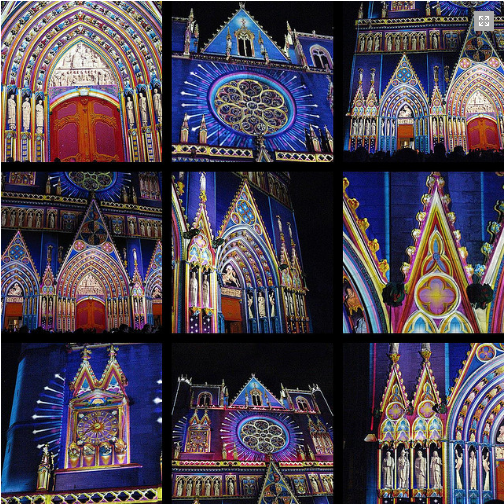
\includegraphics[width=0.6\textwidth]{./Cap1_intro/Fachada1.png}
  \caption[http://www.weltlighting.com/]{Fachada festival Lyon}
  \label{fig:Fachada1}
\end{figure}

\begin{figure}[H]
  \centering
    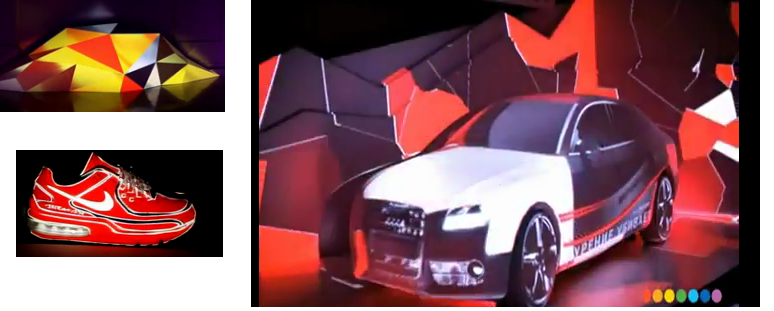
\includegraphics[width=0.75\textwidth]{./Cap1_intro/instalacion3.png}
  \caption[http:\/\/www.youtube.com\/watch?v=1u3p0JEDzcQ\&feature=related ,http:\/\/www.youtube.com\/watch?v=0Lh4OaaYu9E\&feature=related, http:\/\/www.weltlighting.com\/fragment\/]{Instalaciones sobre maquetas.}
  
  \label{fig:Instalacion}
\end{figure}

\begin{figure}[H]
  \centering
    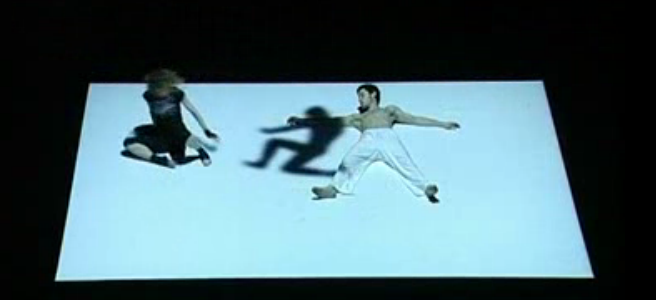
\includegraphics[width=0.75\textwidth]{./Cap1_intro/instalacionHumano1.png}
  \caption[http://vimeo.com/2774865]{Instalación interactiva con actores.}
  \label{fig:Interactiva}
\end{figure}

Para la elaboración de un espectáculo con las características antedichas no existe un procedimiento estándar a seguir sino que cada artista utiliza sus técnicas, métodos y aplicaciones de software que considere adecuadas. No obstante, se identifican etapas comunes como la construcción de un modelo de la escena, la producción del espectáculo y su proyección. A su vez se identifican dificultades comunes como la generación del modelo y la calibración de los proyectores al momento de la reproducción.
En los siguientes capítulos, se estudian distintos métodos para facilitar la obtención del modelo virtual. En particular se relevan métodos de escaneo y reconstrucción de objetos tridimensionales y se implementa una de las estrategias estudiadas para su generación.
Se desarrolla también una aplicación que permite la creación, edición y reproducción de un espectáculo de \emph{video mapping} basada en un motor tridimensional$^\dagger$. Ésta combina la edición y la reproducción permitiendo visualizar en tiempo real los distintos efectos diseñados. A su vez permite distribuir la reproducción entre varias computadoras, asociadas a uno o más proyectores, sincronizadas todas por un componente central.

%Organización del documento: PONER VIÑETAS%
Dicho contenido se concentra en el presente documento, organizado en en cuatro capítulos y cuatro apéndices, cuya temática se detalla a continuación:
\begin{itemize}
\item Capítulo 1 - Introducción a la técnica de \emph{video mapping}.
\item Capítulo 2 - Estado del arte. Explicación de las nociones básicas de la técnica y de las etapas en el proceso de creación: el modelado, la producción y la calibración; presentación de estas dos etapas mediante los enfoques bidimensional y tridimensional; explicación de distintos algoritmos y técnicas para la obtención automática y la reconstrucción de geometría tridimensional.
\item Capítulo 3 - Solución planteada. Presentación de la solución propuesta: una herramienta para la edición y posterior ejecución de espectáculos de \emph{video mapping}.
\item Capítulo 4 - Conclusiones y trabajo futuro. Resumen de las conclusiones y posibles líneas de trabajo futuro.
\item Apéndice A - Relevamiento de aplicaciones de \emph{video mapping}. Presentación de un relevamiento de las aplicaciones existentes más populares, utilizadas para la creación de espectáculos.
\item Apéndice B - Aportes. Presentación de los resultados de una serie de entrevistas realizadas a  \emph{VJs} e ingenieros que contribuyeron a la investigación del estado del arte.
\item Apéndice C - Método de Triangulación. Detalle del método de triangulación utilizado para la obtención automática de geometría tridimensional.
\item Apéndice D - Modelo de Cámara. Explicación de los fundamentos teóricos del modelo de cámara.
\end{itemize}
\clearpage\mbox{}
\chapter{Creación de un espectáculo de \emph{video mapping}}

\section{Introducción}
En la creación de un espectáculo de \emph{video mapping} se identifican tres etapas que son el modelado de la escena, la producción del espectáculo y la proyección del mismo.

En el modelado de la escena se obtiene una representación virtual y abstracta de los objetos reales sobre los que se proyectará. Este modelo será la base para trabajar en posteriores etapas y sobre el cuál se diseñará el espectáculo.

En la siguiente etapa se realiza la producción del espectáculo que consiste en aplicar distintos efectos visuales sobre los objetos modelados y orquestar la ejecución de los mismos. En esta etapa también se diseña y produce la musicalización que será utilizada durante todo el espectáculo.

Es en la proyección del espectáculo en donde se puede contemplar el resultado de los distintos efectos visuales proyectados sobre las superficies acompañados por efectos de sonido.
Para lograr la correspondencia en la proyección de los objetos del modelo con las superficies se debe calibrar la proyección. Esta correspondencia se logra modificando el modelo de la escena, ajustando la posición y orientación de los proyectores, y ajustando los parámetros intrínsecos\footnote{parámetros intrínsecos} de la proyección.

Cada una de estas etapas se puede abordar con un enfoque bidimensional o tridimensional.
Con un enfoque bidimensional el modelo de la escena es una proyección en perspectiva de los objetos a proyectar, por ejemplo, una fotografía. Con un enfoque tridimensional el modelo se mantiene independiente de un punto de vista, representándose con un conjunto de objetos virtuales tridimensionales.

%explicacion de pie de diagrama:redactarlo mejor, El modelo generado en 2d depende del punto de vista del proyector y puede no parecerse a la realidad. El modelo generado 3d se asimila a la realidad y luego con la cámara virtual ajusto el punto de vista del proyector.

\begin{figure}[H]
  \centering
    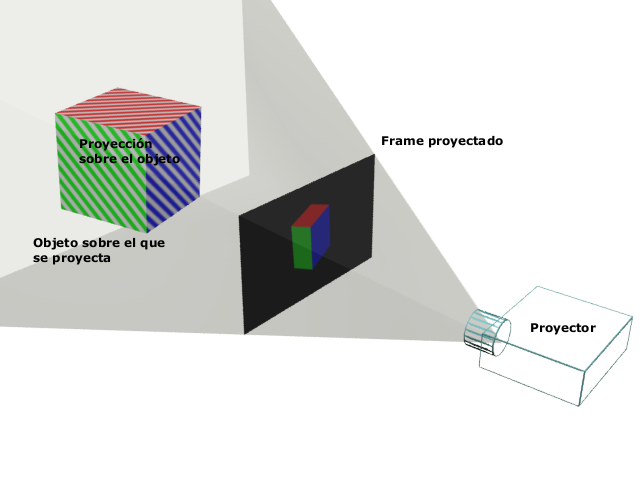
\includegraphics[width=0.7\textwidth]{./Cap2_videomapping/proy2dvs3d}
  \caption{Esquema de proyección.}
  \label{fig:proy2dvs3d}
\end{figure}

\section{Enfoque bidimensional}
\subsection{Modelo}
Un modelo bidimensional refleja lo que vería un observador desde un punto de vista fijo.
%si se quieren agregar hay en el SVN imagenes de proyeccion perspectiva y paralela  VER
Técnicamente es el resultado de una proyección en perspectiva \cite{LibroCompGrafica} sobre un plano de vista de los elementos de la superficie a modelar.

Este punto de vista debe ser considerado al posicionar y orientar el proyector que reproducirá el espectáculo.
La posición, orientación y campo de vista del proyector definirán además la sección de superficie sobre la que se proyectará.
En caso de utilizar más de un proyector cada uno de estos será posicionado en un lugar diferente y por lo tanto será necesario un modelo por cada uno de ellos.

\begin{figure}[H]
  \centering
    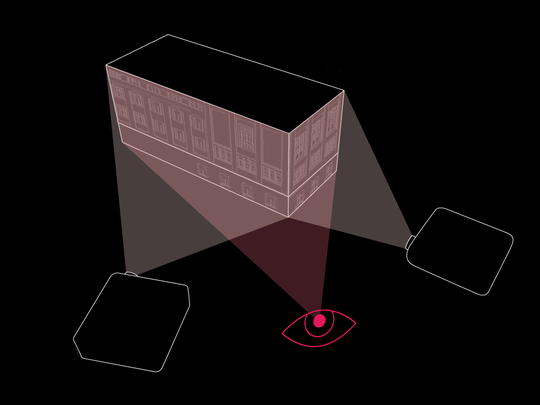
\includegraphics[width=0.7\textwidth]{./Cap2_videomapping/diagrama-2proyectores}
  \caption{Proyectores y sus puntos de vista.}
  \label{fig:diagrama-2proyectores}
\end{figure}

Son ejemplos de modelos una fotografía, un plano arquitectónico de la fachada o figuras geométricas bidimensionales que representan las secciones de las superficies. En algunos casos estos se combinan para obtener como resultado un único modelo.
\begin{itemize}
  \item Una fotografía. Ubicando la cámara de forma que su punto de vista y el del proyector coincidan minimizará los ajustes necesarios en la etapa de calibración.
  \item Un plano arquitectónico contiene información exacta de las medidas de la superficie que representa en una escala dada. Generalmente utiliza el método de proyecciones paralelas \cite{LibroCompGrafica} sobre un plano de proyección. Para utilizar el plano arquitectónico como modelo se debe transformar de forma que coincida con la proyección en perspectiva desde el punto vista que estará ubicado el proyector.
  \item Las figuras geométricas modelan sectores de la superficie donde se proyectará. Un método para generar las figuras geométricas consiste en utilizar un proyector y herramientas de software que permiten delinear el contorno de las secciones de la superficie en tiempo real. Se observa el resultado de cada figura generada proyectada sobre la superficie validando en el momento de la construcción la correctitud del modelo.%%%figuras geometricas queda muy abstracto, hay que llevarlo mas al tema de representacion digital de quads%%%
\begin{figure}[H]
  \centering
    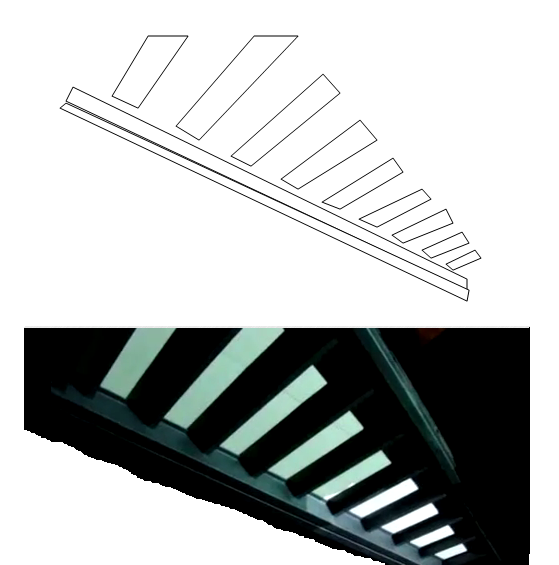
\includegraphics[width=0.7\textwidth]{./Cap2_videomapping/RepresentacionconfigurasGeometricas}
  \caption{Representación con figuras geométricas.}
  \label{fig:RepresentacionconfigurasGeometricas}
\end{figure}

Al usar el proyector para obtener el modelo queda incorporada la perspectiva del mismo y si no se modifica su posición y orientación no sería necesaria la calibración.
Otra opción es dibujar las figuras con una fotografía o plano de fondo, en este caso la construcción de las figuras geométricas se realiza delineando el contorno de la superficie en la fotografía o plano.
Una forma automática de generar el modelo es utilizando técnicas de visión por computadora\footnote{Ver glosario.} en base a algoritmos de reconocimiento de aristas \cite{ArticuloAutom2dmodel}.
\end{itemize}

\subsection{Producción del espectáculo}
La producción del espectáculo en dos dimensiones consiste en definir efectos visuales sobre regiones de un espacio bidimensional discreto\footnote{Ver glosario.} representadas en el modelo de la escena. Este espacio bidimensional discreto se representa con coordenadas de pantalla que identifican cada uno de los píxeles\footnote{Ver glosario.} del área de trabajo. Los efectos visuales se logran realizando cualquier animación computacional que genere una salida gráfica como ser la proyección de videos o imágenes sobre las regiones.
En esta etapa, además de definir los efectos, se planifica en qué momento se mostrarán cada uno de ellos, pudiendo sincronizarse con la música que forma parte del espectáculo.

En computación gráfica se utilizan texturas para proyectar videos e imágenes sobre regiones del área de trabajo. Las texturas son mapas de \emph{bits}\footnote{Ver glosario.} utilizados para cubrir la superficie de un objeto virtual. Estos mapas de \emph{bits} pueden ser generados a partir de imágenes, videos, o incluso dinámicamente mediante algoritmos computacionales permitiendo así crear efectos visuales como por ejemplo la transición de un color a otro.
Cuando se utilizan videos estos pueden ser generados teniendo en cuenta la superficie donde se está proyectando y el punto de vista desde donde se contemplará el espectáculo. Esto es particularmente importante cuando el contenido a mostrar pretende crear una ilusión tridimensional, pues la perspectiva debe coincidir con la de los espectadores.
\begin{figure}[H]
  \centering
    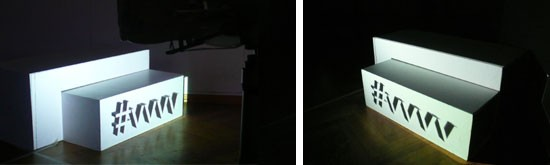
\includegraphics[width=0.7\textwidth]{./Cap2_videomapping/3dillusion}
  \caption{Izq. Ilusión 3D lograda. Der. No se logra la ilusión.}
  \label{fig:3dillusion}
\end{figure}

En este contexto se habla de mapeo, no como la salida a través de un equipo proyector, sino como la operación que logra una correspondencia entre una textura y una figura geométrica que no necesariamente coinciden en tamaño y forma. Para esto se definen coordenadas de textura en cada vértice de la figura geométrica que referencian distintas ubicaciones dentro de la misma.
Las coordenadas de las texturas tienen dos componentes, una horizontal y una vertical llamadas U y V. Si el valor de estas componentes se normaliza entre 0 y 1 entonces la esquina superior izquierda de la textura se corresponderá con la coordenada (0,0), la superior derecha con (1,0), la inferior izquierda con (0,1) y la inferior derecha con (1,1).
%agregar referencia a correspondencia de textura en un objeto, ver para imagen http://en.wikipedia.org/wiki/UV_mapping
Los vértices de una figura geométrica se asocian con coordenadas UV que definen el punto de la textura que se corresponde sobre el vértice. Mediante interpolación se logra mapear toda la textura a la figura geométrica.
Si bien es posible mapear una textura a cualquier figura geométrica, esta correspondencia es más directa utilizando un cuadrilátero ya que a cada uno de los vértices se lo hace corresponder con una esquina de la textura. A su vez el cuadrilátero es la figura básica en las aplicaciones\footnote{Ver sección de aplicaciones relevadas.} de \emph{video mapping}.
Estos cuadriláteros se utilizan como piezas constructoras del espectáculo, cubriendo sectores del modelo sobre los cuales luego se aplican las texturas permitiendo crear los distintos efectos visuales.

\subsection{Calibración}
La calibración se utiliza para ajustar el modelo con la superficie que representa. Inicialmente se fija la posición y orientación del proyector y luego, con ayuda de herramientas de \emph{software}, se aplica la transformación geométrica homografía\footnote{Ver sección Obtención de geometría} a la proyección resultante, para lograr la correspondencia.
En caso de haber modificaciones en la posición y orientación del proyector la calibración deberá realizase nuevamente.
%reescribir esta oración%

Los ajustes necesarios varían dependiendo del método utilizado para obtener el modelo. En caso de utilizar una fotografía, el proyector deberá ser ubicado de forma tal que el punto de vista de la cámara con la que se tomó coincida con el del proyector y así lograr la coincidencia del centro de proyección. Igualmente son necesarios ajustes ya que los lentes de la cámara y el proyector no necesariamente coinciden en el ángulo de visión\cite{LibroCompGrafica2}\cite{LibroPhotographicOptics}. Con el método de generación de figuras geométricas, en el que se modelan las secciones de la superficie a mapear utilizando el mismo proyector, los ajustes se reducen a lograr la misma posición y orientación que tenía el proyector al momento de la captura de secciones, ya que las deformaciones relacionadas a los parámetros intrínsecos fueron implícitamente consideradas durante el proceso de captura.

\section{Enfoque tridimensional}
\subsection{Modelo}
Para el modelado tridimensional se utilizan representaciones de cuerpos y superficies tridimensionales representadas por mallas\footnote{Ver glosario.} de polígonos \cite{Mesh_building}, comúnmente utilizadas en disciplinas como cartografía, visión computacional y computación gráfica. A diferencia de un modelo bidimensional, este no depende de un punto de vista, lo que permite al diseñador visualizar la escena desde diferentes ángulos. Las entidades que conforman la malla son vértices, aristas, caras y atributos numéricos que representan la posición y normales de los vértices, coordenadas de textura y colores. La topología de la malla puede variar, por ejemplo los polígonos que la componen pueden tener distinta cantidad de vértices.

\begin{minipage}{0.35\textwidth}
\begin{flushleft} \large
\begin{figure}[H]
  \centering
    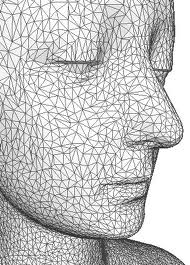
\includegraphics[width=0.7\textwidth]{./Cap2_videomapping/EjemploMallaTriangular}
  \caption{Mallas triangulares.}
  \label{fig:mallas1}
\end{figure}
\end{flushleft}
\end{minipage}
\begin{minipage}{0.45\textwidth}
\begin{flushright} \large
\begin{figure}[H]
  \centering
    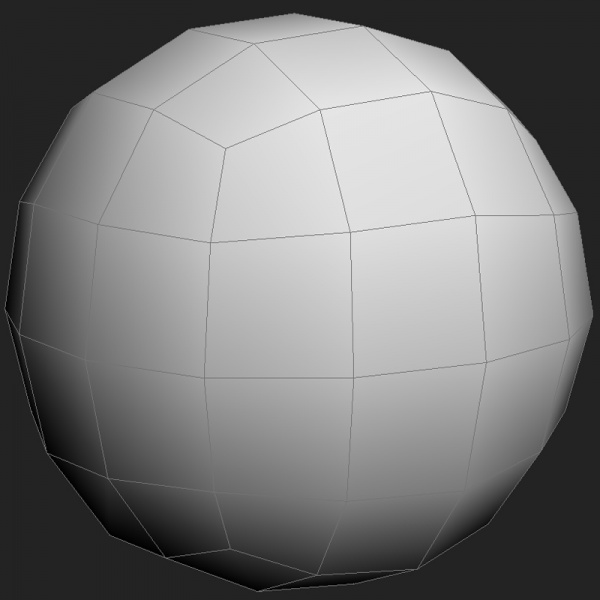
\includegraphics[width=0.75\textwidth]{./Cap2_videomapping/EjemploMalla4Vertices}
  \caption{Mallas de cuadriláteros.}
  \label{fig:mallas2}
\end{figure}

\end{flushright}
\end{minipage}

Las aristas unen los vértices y juntos conforman las caras, y dos caras son adyacentes cuando comparten por lo menos una arista. La valencia de un vértice es el número de aristas en las que participa y el grado de una cara es la cantidad de aristas que la componen.

\begin{figure}[H]
  \centering
    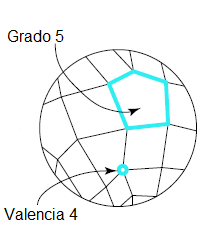
\includegraphics[width=0.35\textwidth]{./Cap2_videomapping/MallaAtributos}
  \caption{Atributos de malla.}
  \label{fig:MallaAtributos}
\end{figure}
Es muy común que las mallas contengan información redundante, para lo que existen técnicas como la de \emph{remeshing} que mediante la utilización de algoritmos específicos reducen la información de la malla sin perder la representatividad de la superficie.
%si se quiere se pone esta referencia:Survey of Polygonal Surface Simplification Algorithms Paul S. Heckbert and Michael Garland doc/papers/Mesh_building/Survey of Polygonal Surface Simplification Algorithms.pdf

Los modelos tridimensionales se generan utilizando distintas técnicas:
%http://en.wikipedia.org/wiki/3D_modeling#Modeling_Process
\begin{itemize}
  \item Modelado utilizando polígonos: a partir de mallas que representan figuras primitivas se podrán construir nuevas mallas, por ejemplo aplicando operaciones de unión o resta.
  %Que es union y resta?%
  También se aplican transformaciones que modifican las aristas, vértices o caras, aproximando el resultado a la superficie que se desea modelar.
  \item  Modelado utilizando curvas: a partir de una jaula creada por curvas se aplican transformaciones para modificarla, manipulando sus puntos de control. Es utilizado en modelado de automóviles, edificios y mobiliario.
  %programas: Maya, 3D Studio Max
  \item Esculpido digital: técnica digital que simula el esculpido convencional, en la que software especializado provee una interfaz para modificar el modelo de forma detallada, oprimiendo y resaltando zonas de la superficie. Es utilizado para lograr efectos especiales en video juegos y películas logrando figuras y texturas complejas.
  %programas: 3D-Coat, Zbrush, y Mudbox
  \item Reconstrucción a partir de fotografías: se obtiene la representación de la superficie mediante mediciones de los objetos fotografiados. Conociendo la escala de la imagen se extrapola y se obtiene la distancia entre dos puntos en la superficie. Es usada en arquitectura, ingeniería, geología, arqueología, etc.
  %esta técnica es llamada fotogrametría en dos dimensiones, estereofotogrametría para obtener información tridimensional
  \item Reconstrucción utilizando hardware especializado: utilizando escáneres tridimensionales se obtiene una nube de puntos\footnote{Nube de puntos} que representa la superficie. Generalemente la cantidad de información obtenida es densa provocando que la información capturada sea redundante. Es por esto que se utilizan algoritmos especializados para reducir la nube de puntos.
  %se puede poner una nota al pie, que esta técnica se ampliará en el capítulo Reconstrucción

\end{itemize}
\subsection{Producción del espectáculo}
La producción del espectáculo en tres dimensiones agrega un nivel de abstracción adicional a la producción bidimensional. Esto permite que el diseñador cree su espectáculo transformando directamente los objetos del modelo tridimensional y no sus perspectivas como en el anterior enfoque.
Esto plantea un cambio en la forma de trabajar en el espectáculo y de planificar la producción, ya que el diseñador no estará restringido a considerar ubicacion alguna de los proyectores. Esta preocupación se traslada a etapas posteriores.

El modo de trabajo se basa en mapear texturas sobre las caras de los objetos tridimensionales de forma análoga a como se realiza sobre figuras bidimensionales. En este tipo de modelos podría ser deseable mapear una textura de forma que abarque varias caras del mismo objeto tridimensional, por ejemplo la superficie de un cilindro. Para lograrlo se deben mapear distintos sectores de la textura en cada una de las caras que conforman la superficie, utilizando coordenadas de textura en cada uno de los vértices. La diferencia está en que en este enfoque los vértices no se encuentran necesariamente en el mismo plano por lo que ajustar una textura bidimensional a este tipo de superficies no es tan directo. Para ello existen técnicas que asisten en la tarea de definir las coordenadas de textura. Una de ellas consiste en aproximar la superficie por una primitiva conocida más simple como puede ser un cubo, cilindro, esfera o plano. Para estas superficies existen funciones matemáticas que proyectan cada punto de la superficie a un plano por lo que se pueden determinar las coordenadas $UV$. Un ejemplo de esto para esferas son las proyecciones utilizadas para representar el planisferio como la proyección cilíndrica equidistante \cite{flatteningTheEarth}. Otra técnica es $UV$ \emph{unwrapping} que consiste en desenvolver los vértices de la superficie, aplanándolos sobre la textura. De esta forma el mapeo se realiza de forma más intuitiva ya que la superficie aplanada es bidimensional al igual que la textura. Esta técnica y las distintas herramientas para ajustar la forma en que se desenvuelve la textura son soportadas por la mayoría de los programas de edición de gráficos tridimensionales.

En la escena tridimensional los objetos son visualizados utilizando cámaras virtuales que fijan un punto de vista. En la salida gráfica se representará entonces la escena desde la perspectiva de una cámara virtual, permitiendo visualizarla desde distintos ángulos. Esto posibilita definir el punto de vista del proyector que reproducirá la salida gráfica, y no se restringe a realizarlo antes de producir el espectáculo sino que una vez producido es posible observar el resultado y elegir el punto de vista que más agrade.
Producir el espectáculo transformando directamente los objetos y no sus perspectivas permite escalar con mayor facilidad en la cantidad de proyectores. Lo único que habría que agregar serían cámaras virtuales que definan más puntos de vista sin modificar el modelo ni los efectos producidos.

Si bien se esta abordando un enfoque tridimensional de la producción del espectáculo, existen casos en que es más sencilla la implementación de ciertos efectos tomando un enfoque en dos dimensiones, sobre todo cuando estos se aplican sobre regiones planas de la superficie. Es por esto que es muy común combinar ambos enfoques y utilizarlos de acuerdo a las necesidades del diseñador. Cabe aclarar que al combinar los enfoques se pierden las ventajas de definir el punto de vista del proyector luego de la producción por lo que los objetos bidimensionales y efectos sobre estos se deben definir una vez fijada la ubicación de los proyectores.

\subsection{Calibración}
Se desarrolla un método de calibración cuyo objetivo es obtener la posición del proyector con respecto a un sistema de coordenadas ubicado en un punto elegido relativo a la escena. Para ello se utiliza una superficie de calibración que puede existir ya en la escena o puede ser ubicada sobre esta de forma temporal. Esta superficie de calibración deberá ser un plano rectangular en donde uno de los vértices será el centro de coordenadas que se desea determinar. La orientación del plano determinará la alineación del centro de coordenadas con sus ejes $X$ e $Y$ alineados con dos de los bordes del plano y el eje $Z$ perpendicular a este. Se utiliza además un proyector asumiendo el modelo \emph{pinhole}\footnote{Pinhole}.

Para encontrar el sistema de coordenadas buscado, se resuelve el problema opuesto que es encontrar la posición del punto que será origen del nuevo centro de coordenadas con respecto al centro de proyección ubicado dentro del proyector. Este método utiliza tres de los vértices de la superficie de calibración que formarán una base del nuevo sistema de coordenadas. Las medidas de la superficie de calibración son conocidas por lo que la distancia entre sus vértices también lo son. Desde el centro del proyector se proyectan rayos de luz, tres de los cuales pasan por los vértices de la superficie de calibración y también por el centro de proyección con coordenadas $(0, 0, 0)$. Para obtener la ecuación de estos rayos solo se precisa un punto distinto al origen. La ecuación de este punto puede ser obtenida utilizando las coordenadas en pantalla del \emph{pixel} que se proyecta en cada vértice de la superficie de calibración.
\begin{figure}[H]
  \centering
    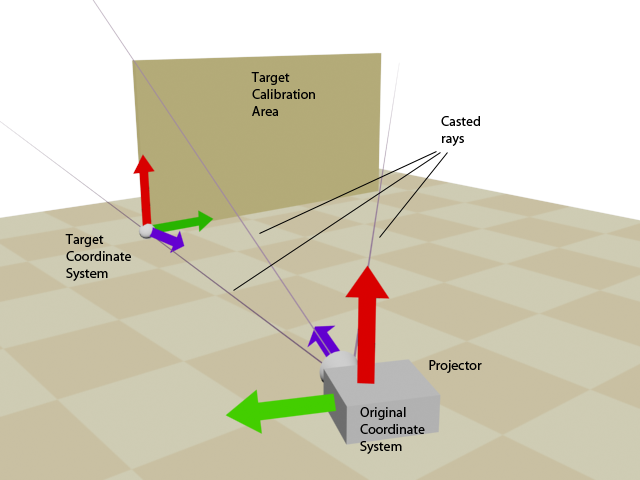
\includegraphics[width=0.7\textwidth]{./Cap2_videomapping/CalibrationSketch}
  \caption{Esquema de calibración.}
  \label{fig:CalibrationSketch}
\end{figure}
Usando las coordenadas en la pantalla de estos puntos y otros parámetros intrínsecos del proyector que son su resolución y el ángulo de proyección, es posible encontrar las coordenadas del punto con respecto al centro de proyección y por tanto la ecuación del rayo.
\[
a(t) = \vec{P} . t,	\mbox{ ecuación del rayo en dónde } \vec{P} \mbox{ es cualquier punto del rayo.}
\]
\[
\begin{cases}
P(X) = \frac{res_x}{2} - s_x \\
P(Y) = \frac{res_y}{2} - s_y \\
P(Z) = \frac{res_y}{2 \cdot \tan \frac{fov_y}{2}}
\end{cases}
\]
en donde $s_x$ y $s_y$ son las coordenadas del \emph{pixel}, $res_x$ y $res_y$ son la resolución horizontal y vertical del proyector y $fov_y$ es el ángulo de proyección vertical del proyector.

Aplicando esta ecuación a cada uno de los puntos a determinar se obtienen las ecuaciones paramétricas de los tres rayos. Vale aclarar que estos puntos $P$ son puntos de los rayos pero no necesariamente coinciden con los vértices de la superficie de calibración. Queda hallar las coordenadas de los vértices determinando el parámetro $t$ para cada ecuación. Para hallar este parámetro se resuelve un sistema de ecuaciones utilizando las tres ecuaciones de los rayos y las distancias conocidas entre estos puntos.
% Sistema de ecuaciones %
\[
\begin{cases}
\lVert{a(t_0) - b(t_1)} = j\rVert \\
\lVert{b(t_1) - c(t_2)} = k\rVert \\
\lVert{c(t_2) - a(t_0)} = l\rVert
\end{cases}
\]
siendo $a$, $b$ y $c$ los rayos y $j$, $k$ y $l$ las distancias entre las parejas de puntos.
La solución será entonces los parámetros $t_0$, $t_1$ y $t_2$ que satisfacen el sistema de ecuaciones no lineal.
Una aproximación a esta solución se puede obtener utilizando métodos numéricos, por ejemplo, el método \emph{trust-region-dogleg}\cite{TrustRegionDogleg}.
Una vez hallados los valores para $t_0$, $t_1$ y $t_2$, las coordenadas de los vértices de la superficie de calibración son $a(t_0)$, $b(t_1)$ y $c(t_2)$.
La base para el sistema de coordenadas con origen en el punto $P$ es:
\[
x' = \frac{b(t_1) - a(t_0)}{\lVert b(t_1) - a(t_0) \rVert},\quad y' = \frac{c(t_2) - a(t_0)}{\lVert c(t_2) - a(t_0)\rVert},\quad z' = -x' \times y'
\]
La ubicación del proyector en este nuevo sistema se obtiene proyectando cualquiera de los rayos en la nueva base de coordenadas.
\clearpage\mbox{}
\chapter{Solución planteada}
\section{Descripción general}%HABLAR QUE VMT SE BASA EN OPENFRAMEWORKS Y OPENGL, QT%
%Mencionar que es nuestra herramienta%
\emph{VMT} es una herramienta para la edición y ejecución de un espectáculo de \emph{video mapping}. Puede utilizar uno o más proyectores eventualmente alejados físicamente unos de otros para lograr cubrir una superficie mayor de la escena a mapear. Para dar soporte al escenario distribuido se cuenta con componentes remotos con el fin de reproducir los efectos y eventos existentes del espectáculo. Mediante un editor tridimensional, es posible observar de forma centralizada lo que se ha producido hasta el momento así como visualizar la salida de cada uno de los proyectores. Si bien es un editor tridimensional se manejan conceptos bidimensionales de capa y cuadrilátero. En \emph{VMT} son llamados \emph{layer} y \emph{quad} respectivamente, y se pueden asociar a una cámara o proyector. La cantidad de estos elementos que se utilizarán en el espectáculo puede ser variada dependiendo del diseño sin existir en \emph{VMT} un límite fijo para ellos. Se proveen mecanismos de calibración diferenciados para objetos tridimensionales y bidimensionales utilizados al trabajar sobre la escena real.

Los efectos de mapeo disponibles son de degradé de colores\footnote{en \emph{VMT} es el efecto \emph{fade}.}, y la aplicación de texturas de imagen o video. Se cuenta además con un efecto para la animación de la posición de los objetos tridimensionales en tiempo de ejecución del espectáculo. Es posible visualizar en todo momento la ejecución de los efectos y su correspondiente impacto en la escena. Los efectos pueden ser lanzados por tiempo, por eventos de teclado o \emph{MIDI}. Se definen en una línea de tiempo navegable, permitiéndose avanzar o retroceder a un intervalo de tiempo dado durante la producción del espectáculo. Una pista de audio puede reproducirse en sincronía con el transcurso de los efectos en el espectáculo.

La interfaz gráfica de usuario está basada enteramente en botoneras y ventanas flotantes para poder tener una vista personalizable y en tiempo real de lo que está sucediendo en la escena. Se proveen mecanismos para almacenar y cargar la definición de la escena utilizando archivos \emph{XML} estándar.

La tecnología de base seleccionada para la creación de los módulos de la herramienta y todas las bibliotecas de terceros que se han utilizado son multiplataforma, lo que permite la compilación y ejecución en entornos \emph{Microsoft Windows}, \emph{Linux} y \emph{Mac OS X}.

\section{Funcionalidades}

\subsection{Manejo de escena y mapeo}

Una escena en \emph{VMT} es una colección de objetos, efectos y cámaras que serán representados gráficamente. Se cuenta con un motor de dibujado que se encarga de generar dicha representación brindando soporte a la visualización de elementos gráficos bidimensionales y tridimensionales en pantalla o proyectados y al mapeo de texturas de imágenes o videos sobre ellos. Este motor ofrece una interfaz genérica para el manejo y edición de objetos y efectos que contiene la escena.

Los elementos bidimensionales \emph{quads} se pueden posicionar en la pantalla de forma tal que al ser proyectados cubran una superficie total o parcial de la escena. Luego, sobre estos \emph{quads} se aplicarán texturas en forma de imagen o video, para que la proyección deforme estas texturas adaptándolas a la forma del \emph{quad}.
Los \emph{quads} también pueden ser utilizados como máscaras para cubrir zonas de otros \emph{quads} o elementos tridimensionales que podrían estar quedando mal proyectadas por deformaciones en la superficie o por ser zonas no deseadas. Una máscara se logra con un \emph{quad} opaco de color negro. Se utiliza el color negro porque es el menos visible al ser proyectado.

Los elementos tridimensionales representan objetos más complejos y ofrecen una mayor versatilidad para realizar mapeos sobre ellos.
El formato estándar utilizado para representar los elementos tridimensionales es \emph{3DS} \cite{3DS} y se permite cargar al motor cualquier geometría que lo respete.
La edición de la geometría de estos objetos tridimensionales es en general un tema complejo pero bien resuelto por varias aplicaciones de edición tridimensional como pueden ser \emph{3D Studio}\footnote{usa.autodesk.com/3ds-max} o Blender\footnote{www.blender.org}. %Por esta y otras razones es que se delega la edición de las formas tridimensionales a programas para este propósito.
Los programas de edición además de permitir modificar la geometría manipulando vértices y caras, también posibilitan la definición de materiales para aplicar propiedades comunes a una cierta selección de caras de la malla tridimensional$^\dagger$. \emph{VMT} utiliza estas selecciones de caras para mapear texturas sobre ellas resolviendo de esta forma el mapeo en tres dimensiones.

El mapeo tridimensional se realiza básicamente definiendo las coordenadas \emph{UV} en cada vértice del modelo. Las aplicaciones de edición tridimensional antes mencionadas proveen herramientas para hacer esta tarea de forma muy intuitiva. Ejemplo de esto es la definición de coordenadas de mapeo de un cilindro para mapear una textura en una columna cilíndrica.
Los elementos gráficos por sí mismos no son representables siendo necesario asignarles un material y es a este material que se le asigna un color o una textura con la cual se representará el objeto.
En la implementación de los materiales se utilizan \emph{shaders} que son programas que se ejecutan en los procesadores gráficos y tienen como ventaja que son altamente paralelizables, permitiendo realizar cálculos de forma más rápida y eficiente. En la aplicación se utiliza el lenguaje de shaders para \emph{OpenGL} GLSL\cite{GLSL} para la implementación de un shader básico que combina una textura de imagen o video con un color para obtener el resultado visible del material. Este color tiene un canal alfa$^\dagger$ y por lo tanto se pueden lograr texturas y colores con niveles de transparencia.

Para visualizar los elementos tridimensionales es necesario definir un punto de vista. Esto se logra mediante el agregado de una cámara en el motor y la configruación de sus propiedades, entre ellas su ubicación o punto de vista. Los proyectores con los que se realiza el espectáculo de \emph{video mapping} son también representados como cámaras en el motor, pero no toda cámara configurada representa un proyector, ya que se pueden contar con cámaras que representen puntos de vista de un observador del espectáculo que sea de interés para el creador.
Las cámaras permiten ajustar sus parámetros mediante operaciones comunes a cámaras virtuales de forma similar a lo que ocurre en otros paquetes de animación por software y a cámaras cinematográficas en general. Estas operaciones representan movimientos de la cámara llamados \emph{Roll}, \emph{Orbit}, \emph{Dolly} y \emph{Pan}. \emph{Roll} se refiere al movimiento en donde la posición de la cámara y el punto de vista son fijos y ésta rota a través del eje formado por ellos. \emph{Orbit} es cuando la cámara orbita alrededor de su punto de vista, es decir, la posición de la cámara cambia pero siempre visualizando el mismo punto y manteniendo la distancia a este. \emph{Dolly} es el movimiento en donde se mantienen el punto y la dirección de vista pero se mueve la posición de la cámara acercándose y alejándose del objetivo. Por último, \emph{Pan} es el tipo de movimiento en el cual se mueve la cámara cambiando la posición y el punto de vista y siempre manteniendo un paralelismo con la dirección.
%Mencionar que son las transformaciones estandar de camaras%

\begin{figure}[H]
  \centering
    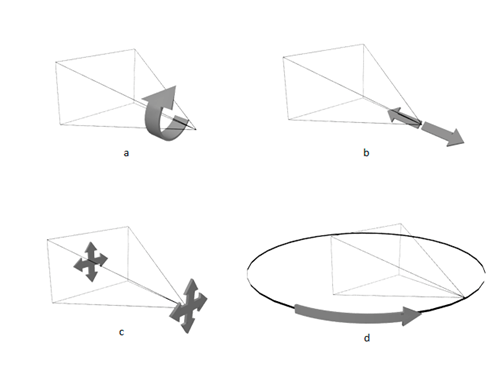
\includegraphics[width=0.5\textwidth]{./Cap5_vmt/vmtengine-cameramove.png}
  \caption{Movimientos de cámara. a) \emph{Roll} b) \emph{Dolly} c) \emph{Pan} d) \emph{Orbit}}%imagen nuestra no hay que referenciar%
  \label{fig:VMT-CameraMove}
\end{figure}

Aparte de estos parámetros de ubicación, también existe el parámetro \emph{Field Of View (FOV)} o campo de vista que es el ángulo de apertura de la cámara. Para el caso de cámaras que representan proyectores, este parámetro debe coincidir con el ángulo de apertura del proyector para ajustar correctamente las escenas con respecto a lo que muestra la cámara en pantalla.
Mediante estas operaciones es que las cámaras virtuales de \emph{VMT} ajustan sus parámetros para que la proyección de objetos tridimensionales coincida con las superficies proyectadas.
Hay que destacar que las cámaras proveen un punto de vista solo para los elementos tridimensionales. Los \emph{quads}, que como se mencionó son contrucciones bidimensionales, no dependen del punto de vista de la cámara y se representan en un sector de la pantalla relativo a esta. Es por esto que los \emph{quads} no alteran su posición en pantalla al ajustar los parámetros de la cámara.

Los \emph{quads} se pueden organizar en grupos, y estos pertenecen a una o más capas. A su vez cada capa pertenece a una única cámara de manera de representar las zonas a cubrir por un solo proyector. Es posible aplicar una transformación inicial a una capa, la que se aplicará a todos los \emph{quads} o grupos de \emph{quads} contenidos en ella. Esto es útil para ajustar la proyección de los \emph{quads} en caso de mover el proyector levemente y que esta proyección deje de coincidir con las superficies, y provee la funcionalidad básica y de bajo nivel para el mecanismo de calibración bidimensional que se detallará más adelante.

Las texturas se asocian a grupos de \emph{quads}. Los grupos también permiten variar de forma limitada como se mapean las texturas a los \emph{quads} que los componen. Pueden ser mapeadas por cara en donde a cada uno de los \emph{quads} se le mapeará toda la textura, o también de forma plana, esto es que la textura sea mapeada al conjunto entero de \emph{quads} como si estos fueran trozos de un \emph{quad} de mayor tamaño.

\begin{figure}[H]
  \centering
    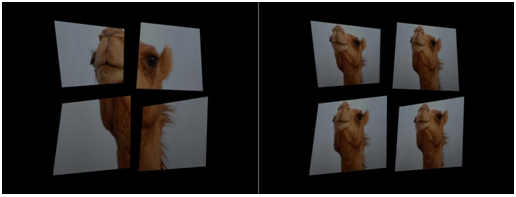
\includegraphics[width=0.7\textwidth]{./Cap5_vmt/vmtengine-maping.png}
  \caption{Izquierda: Proyección plana. Derecha: Proyección por cara.}%imagen nuestra no hay que referenciar%
  \label{fig:VMT-Projection}
\end{figure}

Con estas variantes de proyección se le dan más posibilidades a un artista para lograr los efectos utilizados normalmente en espectáculos de \emph{video mapping}.

La escena también contiene los efectos que se ejecutarán durante el espectáculo. Se aceptan como efectos la asignación de texturas en forma de imagen o video, ya sea a grupos de \emph{quads} u objetos tridimensionales, el \emph{fade} en un material desde un color inicial a otro final, y la animación de la posición de un objeto tridimensional de un origen a un destino en un lapso de tiempo dado.

El efecto de mapeo de texturas es el más básico pero también el más potente en cuanto a la gran cantidad de alternativas al momento de mapear texturas sobre superficies. La variedad y la complejidad de las texturas está en la creación de los recursos de imagen o video que se deseen mapear. Al permitirse mapear estas texturas sobre objetos tridimensionales no es necesario distorsionar la forma de los videos sino que será el motor quien los adaptará a la forma del objeto que está siendo mapeado. El efecto de \emph{fade} puede ser combinado en un objeto que ya disponga de una textura y así permitir por ejemplo su atenuación o resaltado. La duración del \emph{fade}, al igual que la de animación de posición, es configurable.

Cabe aclarar que el estado final de la escena y todos los objetos contenidos en ella será el que resulte luego de la finalización de los efectos. Por ejemplo, si un objeto es de color rojo, y tiene un efecto de \emph{fade} al azul aplicado, su color luego de la ejecución del efecto continuará siendo azul.

Como se mencionó anteriormente, una de las tareas principales es la representación en pantalla o la proyección de los elementos gráficos. La implementación del dibujado se realiza en un bucle principal de la aplicación encargado de actualizar todos los objetos de la escena de ser necesario, procesar los eventos pendientes y finalmente dibujar el resultado. Este es un proceso cíclico que se repite varias veces por segundo.
En cada uno de estos ciclos se generan los cuadros que son las imágenes que se muestran como resultado final.
Para dar la ilusión de continuidad, la frecuencia de estos ciclos debe ser alta. En el caso de \emph{VMT} ésta se predetermina en 60 ciclos por segundo aunque alcanzar esta frecuencia dependerá de varios factores como la cantidad de \emph{quads}, tamaño de texturas utilizadas, capacidad de procesamiento y memoria de los equipos.
Si esta frecuencia se encuentra muy por debajo de los 60 ciclos, la reproducción del espectáculo no será fluida y se podrán percibir saltos o pausas al reproducirlo.
Para que esta frecuencia efectivamente se logre es necesario que el procesamiento de cada uno de los ciclos del bucle principal sea eficiente en cuanto al costo de procesamiento en cada tarea u operación. A continuación se muestra un pseudo-código del bucle principal de dibujado y se analizan cada una de las acciones que se toman, su impacto en cuanto al rendimiento del programa y las medidas que se tomaron para su optimización:

\begin{algorithm}
    \caption{Pseudo-código bucle de dibujado.}
    \label{alg:mainLoop}
    \begin{algorithmic}
      \State $posicionarCamara();$
      \ForAll{objeto3d $obj$ en la escena}
        \ForAll{cara $c$ de $obj$}
             \State $mat = cargarMaterial(obj);$
             \State $c.dibujar(mat);$
         \EndFor
      \EndFor

      \State $resetCamara();$
      \ForAll {quad $q$ en la escena}
         \State $mat = q.cargarMaterial();$
         \State $q.dibujar(mat);$
      \EndFor
    \end{algorithmic}
\end{algorithm}


Un bucle de este estilo cuenta con varios cuellos de botella.
La carga de materiales implica copiar una textura a la zona de la memoria de video correspondiente para utilizarla. Esto podría ser un proceso lento si no se disponen las texturas precargadas en memoria. Es por esta razón que las texturas se cargan desde un comienzo en memoria y luego se utilizan referencias para identificarlas y asociarlas a una unidad de textura de \emph{OpenGL}\footnote{www.opengl.org/wiki/Texture} para que se encuentre disponible.
Otra optimización pasa por hacer uso de \emph{shaders} para el cálculo del resultado visual final.
La visualización fluida de un espectáculo de \emph{video mapping} es difícil de predecir ya que, como se puede ver en el pseudo-código, los tiempos de ejecución dependen de la cantidad de materiales, caras, objetos y \emph{quads} incluidos en la escena.
Si se utilizan videos en las texturas, la compresión y resolución de estos también afecta la fluidez del espectáculo. Preferentemente deberían estar descomprimidos o con una baja tasa de compresión. El mismo problema ocurre con formatos de imágenes comprimidas, pero teniendo un menor impacto en el rendimiento de la reproducción del espectáculo.
%Esto no es verdad ya que hay codecs que son ideales para real time%

\subsection{Multi proyector}

Uno de los puntos fuertes de \emph{VMT} es la posibilidad de editar y visualizar un espectáculo de \emph{video mapping} utilizando más de un proyector. El soporte de múltiples proyectores puede lograrse de diferentes formas de distribución.

La forma más sencilla de conectar varios proyectores es con más de una salida de video desde la mismo computadora. Esto es posible mediante una tarjeta de video con salida múltiple, conectando cada proyector a cada una de estas salidas. Luego, se configura el sistema operativo para que extienda la resolución en las múltiples salidas y de esta forma se dispondrá de un área de trabajo mayor. Los diferentes sectores del área de trabajo serán desplegados por los proyectores conectados.
\emph{VMT} permite, al inicio de un espectáculo, indicar la resolución y la posición en pantalla en donde se desplegará. Controlando estos parámetros se permiten distintas variaciones en la configuración de la aplicación y en la disposición de los proyectores.

Otra forma de lograr varias salidas es conectando un dispositivo como las tarjetas \emph{DualHead2Go} o \emph{TripleHead2Go}\footnote{www.matrox.com/graphics/en/products/gxm/} y de esta manera conectar dos o tres proyectores a partir de una única salida de la tarjeta de video. El resultado es similar al anterior, extendiendo el área de trabajo a la resolución duplicada o triplicada.

Estas variantes en la forma de conectar los proyectores son útiles cuando se desea proyectar sobre una superficie tan extensa que un solo proyector no pueda abarcarla completamente, ya que como se menciona, el área de trabajo o escritorio es extendido para abarcar la cantidad de proyectores conectados al computador único, con la restricción de que están todos organizados de forma contigua. En cambio, si queremos proyectar sobre zonas de la escena contiguas entre si, lo ideal es contar con proyectores conectados a nodos distribuidos e independientes tanto al momento de la producción del espectáculo como al de su ejecución.

\begin{figure}[H]
  \centering
    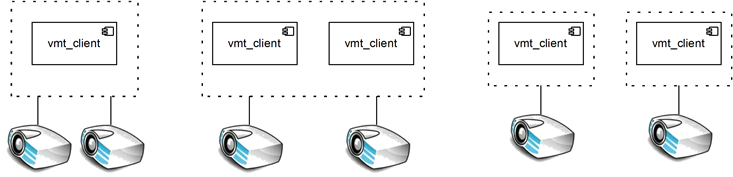
\includegraphics[width=0.8\textwidth]{./Cap5_vmt/vmt_multiProjector.png}
  \caption{Escenarios posibles de múltiples proyectores en VMT}%imagen nuestra no hay que referenciar%
  \label{fig:VMT-MultiProjector}
\end{figure}


En \emph{VMT}, el escenario descrito se implementa teniendo una instancia de \emph{VMT} maestro que orquestará toda la ejecución del espectáculo, y varias instancias de \emph{VMT} esclavo con uno o mas proyectores conectados. Para modelarlo en la herramienta se agregan los proyectores a la escena, asignando las propiedades para cada uno en particular, y luego se define la red de nodos de \emph{VMT} esclavo con la información de conectividad necesaria y su asociación al proyector que tiene conectado el nodo. La comunicación entre maestro y esclavos se realiza sobre \emph{OSC}, protocolo construido sobre \emph{UDP} para \emph{IP} vía \emph{Ethernet} o \emph{WiFi}. Por la naturaleza del protocolo \emph{UDP}, es preferible contar con conexiones cableadas en lugar de inalámbricas dada la alta tasa de pérdida de paquetes que existe en este tipo de redes, lo cual podría causar desincronización de algunos nodos esclavos. \emph{OSC} también permite a cualquier aplicación capaz de enviar mensajes \emph{OSC} y que conozca el formato de los mismos para \emph{VMT}, controlar los esclavos y por consiguiente lo que se proyecta en los correspondientes proyectores.

%%% VA ACÁ Esta información es necesaria para establecer el canal de comunicación con el proceso remoto y deducir que información se enviará al nodo en base a su cámara asociada. Recordar que las \emph{layers} están asociadas a una y solo una cámara, por lo cuál si un efecto está aplicado sobre un \emph{quad} o grupo de \emph{quads}, el mismo deberá ser propagado al nodo cuya cámara sea la que los contiene. Referente a los efectos aplicados sobre objetos tridimensionales, estos serán enviados a todos los nodos ya que todas las cámaras tienen visibilidad de la escena tridimensional, aunque esta sea desde perspectivas diferentes.

\subsection{Calibración}

\emph{VMT} ofrece la capacidad de calibrar las cámaras para que la proyección reflejada por los proyectores se corresponda y ajuste a la geometría de la escena.
Como se mencionó anteriormente, \emph{VMT} permite trabajar simultáneamente de forma bidimensional y tridimensional. Cada uno de estos modos de trabajo requiere distintos mecanismos de calibración.

La calibración bidimensional se basa en ajustar todos los \emph{quads} de una \emph{layer} de forma conjunta.
Inicialmente, al preparar el espectáculo, los \emph{quads} son posicionados en pantalla para cubrir las áreas de interés a proyectar. Luego de este posicionamiento inicial, cualquier movimiento de los proyectores causará que se desajuste simultáneamente la proyección de todos los \emph{quads}. Si ocurre un desajuste se hace necesario reposicionar los \emph{quads} para que vuelvan a cubrir las áreas a proyectar.
\emph{VMT} ofrece la posibilidad de ajustar todos los \emph{quads} pertenecientes a una misma \emph{layer} de forma simultánea aplicando una homografía. Esta transformación es la que ocurre naturalmente en la proyección al variar la posición u orientación del mismo por lo tanto es necesario aplicar la transformación inversa para que los \emph{quads} se ajusten nuevamente a las superficies.

Por otra parte, la calibración tridimensional se basa en hacer coincidir los parámetros de posición, orientación y proyección de las cámaras con los de los proyectores físicos. Este ajuste de parámetros se realiza manualmente por el usuario, utilizando los modos de movimientos de cámara antes mencionados. Esta calibración es necesario hacerla de forma independiente en cada una de las cámaras y proyectores.

Cabe acotar que en los escenarios de múltiples proyectores este modelo de calibración asume que existe un solo proyector conectado a cada nodo, si bien es posible conectar más de uno mediante placas especializadas como se vio anteriormente. Sólo se podrán modificar los parámetros a la única cámara asociada al nodo en el modelo \emph{VMT}, por lo cuál en caso de ser más de un proyector no será posible ajustar los parámetros de todos. Los planos de imagen tampoco podrían coincidir, si no están posicionados exactamente paralelos.


\section{Interfaz gráfica de usuario}

Para la estructura definida de escena o espectáculo, la interfaz gráfica cuenta con formularios sencillos de altas, bajas y modificaciones para todos los tipos de objetos existentes. Se diseñó en base a barras de herramientas flotantes de forma de poder tener visibilidad de la escena en todo momento y observar así como los cambios efectuados impactan sobre ella.

\begin{figure}[H]
  \centering
    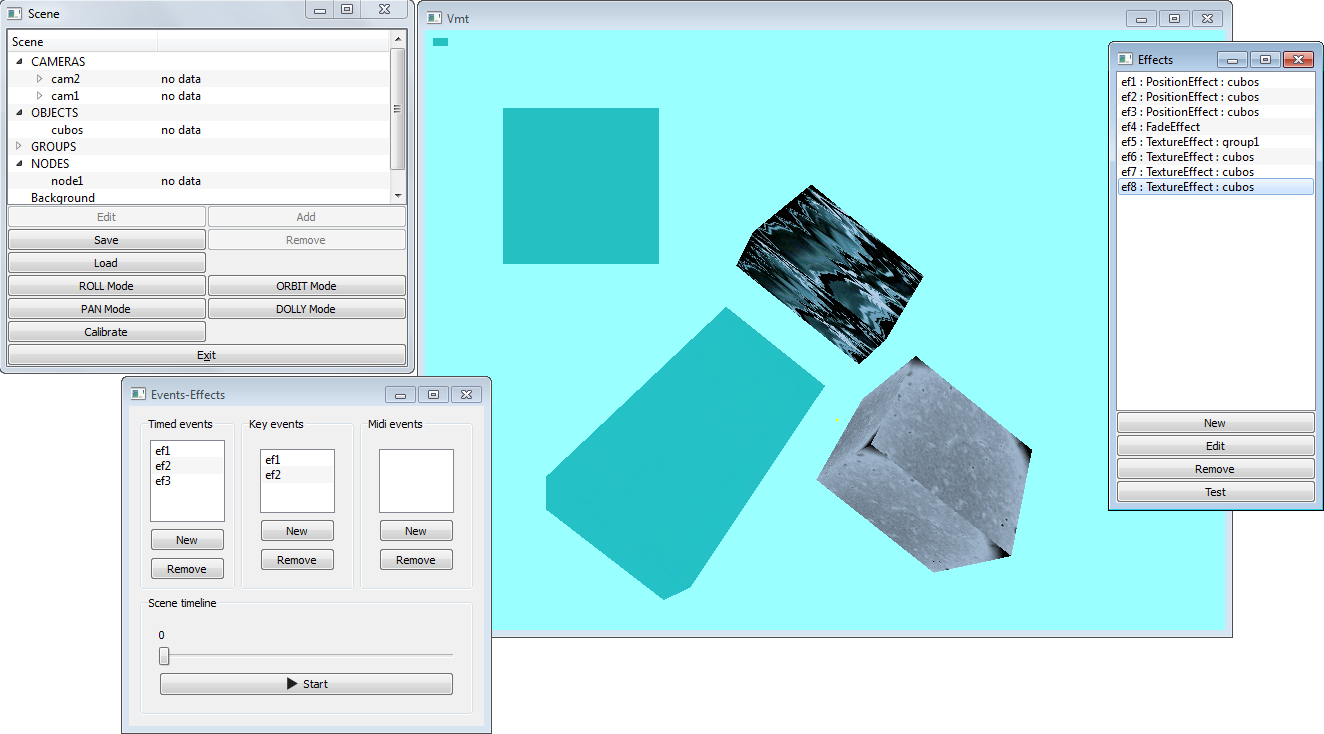
\includegraphics[width=0.8\textwidth]{./Cap5_vmt/vmt_todo.png}
  \caption{Vista general de la interfaz de usuario de \emph{VMT}}
  \label{fig:VMT-MainWindow}
\end{figure}

Al inicio se cuenta con una vista gráfica de la escena desde el punto de vista de la cámara activa, una vista de los objetos contenidos en la escena, la lista de definición de efectos y una línea de tiempo con las listas de efectos por tiempo, por evento de teclado y evento \emph{MIDI}.
En la ventana de escena se manejan los objetos bidimensionales y tridimensionales, cámaras, luces, capas y los nodos distribuidos del espectáculo. También es desde donde se ejecuta la calibración de las cámaras virtuales. En la visualización de la escena se ofrecen diferentes modos de cámara que permite girar u orbitar alrededor del centro, o moverse en cada uno de los ejes.

\begin{figure}[H]
  \centering
    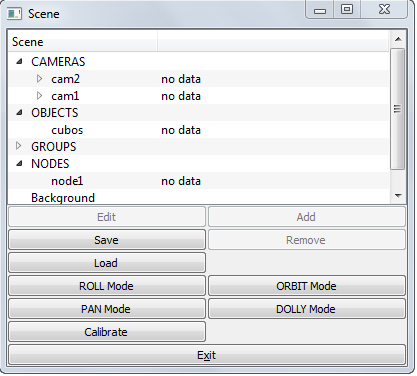
\includegraphics[width=0.5\textwidth]{./Cap5_vmt/vmt_scene.png}
  \caption{Ventana para manejar la escena}
  \label{fig:VMT-SceneWindow}
\end{figure}

\subsection{Cámaras, capas y \emph{quads}}
Las cámaras tienen todas las propiedades usuales que se pueden encontrar en paquetes de \emph{software} de animación tridimensional como ser posición, \emph{eye}, \emph{up}, \emph{FOV}, aspecto, \emph{near}\footnote{explicar near}, \emph{far}\footnote{explicar far}.

\begin{figure}[H]
  \centering
    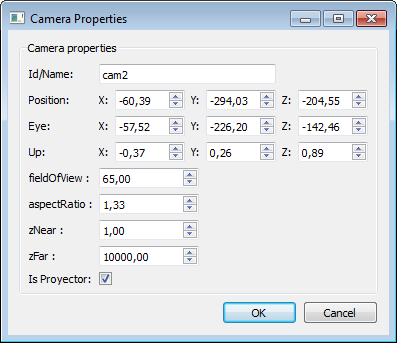
\includegraphics[width=0.5\textwidth]{./Cap5_vmt/vmt_cameraProperties.png}
  \caption{Diálogo de propiedades de cámara}
  \label{fig:VMT-CameraProperties}
\end{figure}

Las cámaras y proyectores son modeladas con el elemento cámara diferenciando mediante la propiedad \emph{isProjector}. De esta forma un elemento cámara se utiliza para simular la vista de un observador, mientras que un proyector será la vista de la proyección en perspectiva del espectáculo.
Los tipos de movimiento de la cámara activa son los descriptos anteriormente.

\begin{figure}[H]
  \centering
    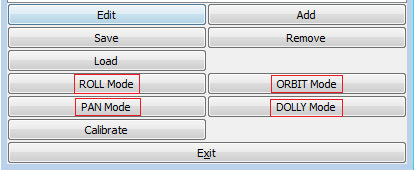
\includegraphics[width=0.5\textwidth]{./Cap5_vmt/vmt_SceneBotonera.png}
  \caption{Acciones para seleccionar modo de movimiento de la cámara activa}
  \label{fig:VMT-CameraActions}
\end{figure}

Una vez seleccionado el modo de la cámara, manteniendo presionado el botón izquierdo del ratón al moverlo se mueve la cámara acorde al modo seleccionado.
Cada cámara es a su vez un contenedor de \emph{layers}. Su propósito es manejar todo lo relacionado al mapeo sobre estructuras bidimensionales, y por ello son los contendores de \emph{quads} bidimensionales sobre los cuales se pueden realizar todas las operaciones y efectos disponibles.

\begin{figure}
	\begin{center}
		\begin{tabular}[c]{cc}
			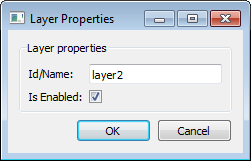
\includegraphics[width=0.3\textwidth]{./Cap5_vmt/vmt_layerProperties.png}
				&        
			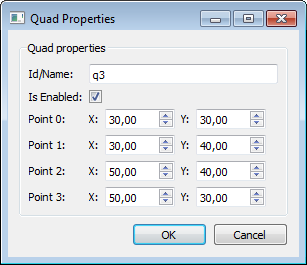
\includegraphics[width=0.3\textwidth]{./Cap5_vmt/vmt_quadProperties.png}
		\end{tabular}
	\end{center}
	\caption{Propiedades de los objetos \emph{Layer} y \emph{Quad}}
	\label{fig:VMT-LayerQuadProperties}
\end{figure}

Tanto el \emph{quad} como la \emph{layer} tienen propiedades editables en tiempo de edición o durante el espectáculo para mostrarse u ocultarse completamente. Si se oculta una \emph{layer}, todos los \emph{quads} contenidos en ella también serán ocultados. En caso de mostrarla, todos los \emph{quads} visibles volverán a desplegarse.

\subsection{Objetos tridimensionales}

Se permite agregar a la escena objetos tridimensionales con formato de malla triangular del tipo \emph{3DS}.

\begin{figure}[H]
  \centering
    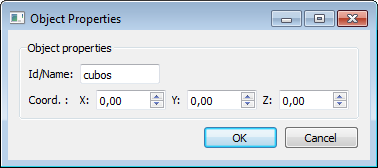
\includegraphics[width=0.5\textwidth]{./Cap5_vmt/vmt_objectProperties.png}
  \caption{Diálogo de propiedades de objeto tridimensional}
  \label{fig:VMT-ObjectProperties}
\end{figure}

\subsection{Efectos}

Se proveen ventanas flotantes tanto para la definición de efectos como para la asociación con sus disparadores como ser un instante específico, un evento de teclado o un evento \emph{MIDI}.

Si un efecto es definido para ser desplegado en un instante dado este se podrá visualizar cuando la línea de tiempo pase por ese instante. En caso de ser definido por evento este será visualizado cada vez que el evento asociado suceda, sea un evento de teclado o \emph{MIDI}.
Los efectos de posición son aplicables únicamente a objetos tridimensionales y permiten animar el objeto trasladándolo de una posición inicial a una final.

\begin{figure}[H]
  \centering
    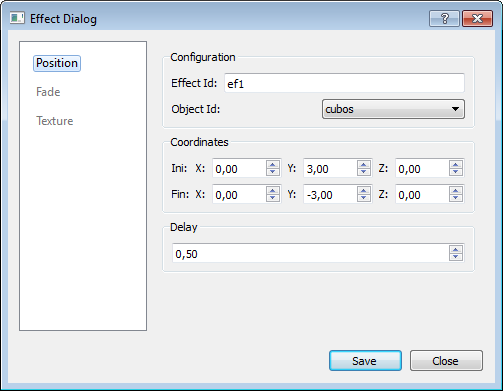
\includegraphics[width=0.5\textwidth]{./Cap5_vmt/vmt_EfectDialog1.png}
  \caption{Diálogo de definición de efecto de tipo posición}
  \label{fig:VMT-EffectPossition}
\end{figure}

Los efectos de \emph{fade} sólo son aplicables a grupos de \emph{quads} y lo que permiten es pintar todos los \emph{quads} del grupo de un color inicial e ir pasando por toda la gama de colores intermedios hasta llegar al color final. Para la selección de colores se utiliza un diálogo específico para ese propósito. También es posible definir la duración del efecto.

\begin{figure}[H]
  \centering
    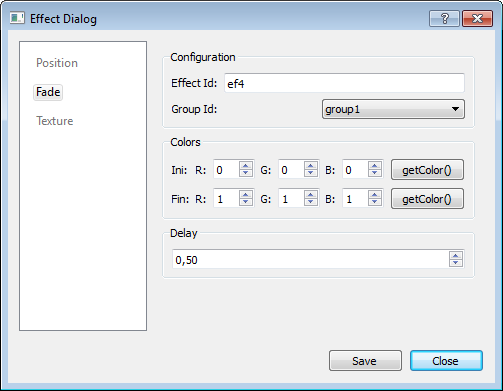
\includegraphics[width=0.5\textwidth]{./Cap5_vmt/vmt_EfectDialog2.png}
  \caption{Diálogo de definición de efecto de tipo \emph{fade}}
  \label{fig:VMT-EffectFade}
\end{figure}

Los efectos de tipo textura son aplicables tanto a grupos de quads como a objetos tridimensionales. Se pueden definir texturas de tipo Imagen o Video. En ambos casos es necesario proporcionar el camino al archivo multimedia correspondiente. Para el caso especifico de un efecto de textura asociado a un objeto tridimensional, es necesario proporcionar además la cara o conjunto de caras sobre los cuales se va a mapear el efecto de tipo textura definido.

\begin{figure}[H]
  \centering
    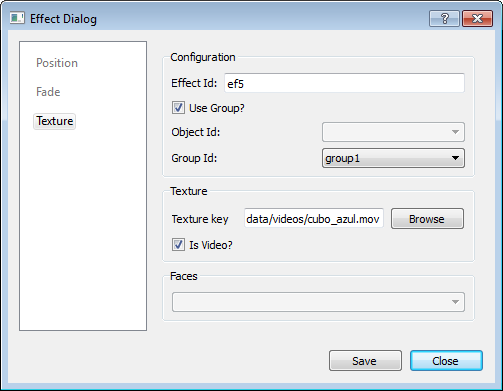
\includegraphics[width=0.5\textwidth]{./Cap5_vmt/vmt_EfectDialog3.png}
  \caption{Diálogo de definición de efecto de tipo textura aplicada a un grupo.}
  \label{fig:VMT-EffectTexture}
\end{figure}

\begin{figure}[H]
  \centering
    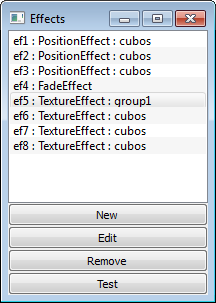
\includegraphics[width=0.2\textwidth]{./Cap5_vmt/vmt_Efects.png}
  \caption{Lista de efectos definidos en la escena}
  \label{fig:VMT-EffectList}
\end{figure}

Es posible visualizar el efecto que se está creando presionando el botón \emph{Test} de la lista de efectos. Esto disparará la ejecución por una única vez del efecto seleccionado en la lista.

\subsection{Calibración}

El proceso de calibración en \emph{VMT} se basa en posicionar cuatro puntos de la superficie donde se proyecta y cuatro puntos de la capa contenedora de \emph{quads} para de esta forma calcular la matriz de transformación de la homografía que los hace corresponder.

\begin{figure}[H]
  \centering
    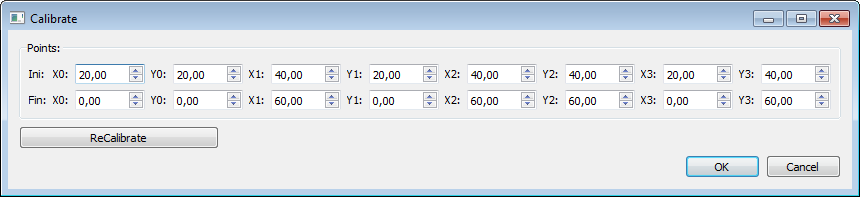
\includegraphics[width=0.6\textwidth]{./Cap5_vmt/vmt_Calibrate.png}
  \caption{Diálogo para configurar y ejecutar la calibración}
  \label{fig:VMT-Calib}
\end{figure}

Al ingresar en el modo calibración se muestra en la pantalla de edición cuatro puntos azules de destino y cuatro puntos rojos de origen junto con el diálogo de configuración de la calibración.
El diálogo posee controles para posicionar cada uno de los ocho puntos mostrados en pantalla. Se deberán posicionar los cuatro puntos de origen en regiones significativas de la capa donde hayan vértices de \emph{quads} preferiblemente alejados entre si. De esta forma se minimiza el error obtenido al calcular la matriz.
Los cuatro puntos de destino se deberán posicionar observando la proyección de estos sobre la superficie. Una vez los ocho puntos estén posicionados se podrá calcular y aplicar la nueva matriz de calibración presionando el botón \emph{OK}.
Mediante el botón \emph{ReCalibrate} se reestablece la calibración original, descartando los cambios realizados.

\subsection{Línea de tiempo}

Tanto para la fases de producción y previsualización del evento como para la ejecución o reproducción del espectáculo en vivo, es necesario contar con controles para el manejo de la línea de tiempo.

\begin{figure}[H]
  \centering
    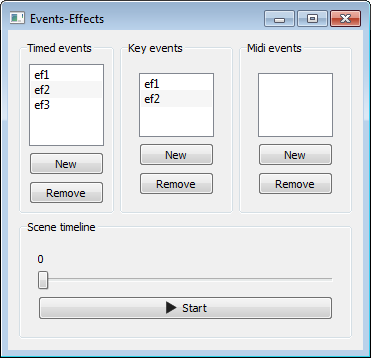
\includegraphics[width=0.5\textwidth]{./Cap5_vmt/vmt_events_effects.png}
  \caption{Diálogo con línea de tiempo y lista de efectos asociados a tiempo y eventos}
  \label{fig:VMT-Timeline}
\end{figure}

La aplicación provee una forma de iniciar el evento mediante la acción de \emph{Start}. Se provee una vista gráfica representada con una barra deslizante y una vista numérica para reflejar el avance en el tiempo en relación a la duración total del evento. Utilizando la barra deslizante es posible navegar por la línea de tiempo e iniciarla visualización del evento desde un instante cualquiera. Esto último es muy útil para la fase de pre-producción del espectáculo en la cual es muy común que el usuario se quiera concentrar en un lapso específico en el que se está trabajando.

Sobre la línea de tiempo se pueden observar las listas de eventos agrupados por tipo, pudiéndose asociar cualquiera de los eventos previamente definidos a un instante dado o a un código de evento a ser utilizado durante el espectáculo, ya sea de teclado o proveniente de dispositivos de entrada \emph{MIDI}.

\subsection{Nodos remotos}

Para modelar la red de nodos esclavos de \emph{VMT} en los cuales se conectarán proyectores remotos es preciso definir, para cada nodo, su dirección \emph{IP} y número de puerto en donde estarán configurados así como también la cámara definida en la escena que representará al proyector asociado.

\begin{figure}
	\begin{center}
		\begin{tabular}[c]{cc}
			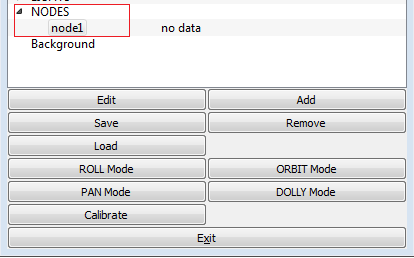
\includegraphics[width=0.3\textwidth]{./Cap5_vmt/vmt_nodeProperties_1.png}
				&        
			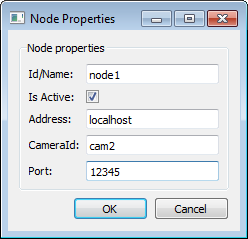
\includegraphics[width=0.3\textwidth]{./Cap5_vmt/vmt_nodeProperties_2.png}
		\end{tabular}
	\end{center}
	\caption{Lista de nodos y diálogo de propiedades de nodos}
	\label{fig:VMT-Nodes}
\end{figure}

\subsection{Escena en XML}
Se permite almacenar en archivos \emph{XML} estándar una representación de lo que se ha definido en la escena. Para la búsqueda de los archivos \emph{XML} se utilizan diálogos nativos para este propósito.

\begin{figure}[H]
  \centering
    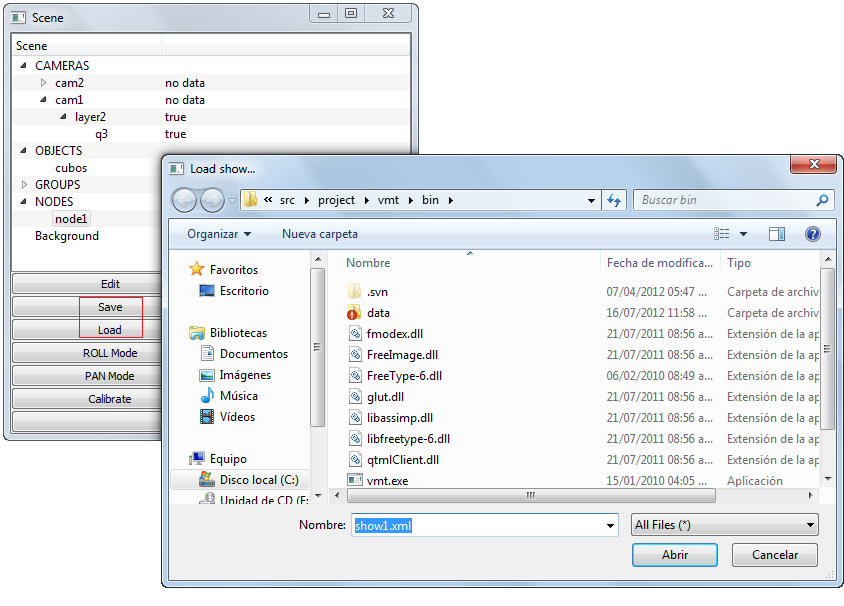
\includegraphics[width=0.5\textwidth]{./Cap5_vmt/vmt_loadShow.png}
  \caption{Diálogo para cargar y guardar archivos \emph{XML}.}
  \label{fig:VMT-XML}
\end{figure}

\section{Decisiones de implementación}
Para la implementación del módulo de interfaz gráfica se siguió el patrón \emph{Model-View-Controller (MVC)}\footnote{Explicar MVC}. Para cada ventana se generaron modelos que manejan los datos relevantes a cada una, impactando en el modelo general de la aplicación en caso de ser necesario.
Se utilizó \emph{Qt Framework} \cite{Qt-framework} como biblioteca de base para la creación de las ventanas, sus controles gráficos y manejo de la comunicación que ocurre entre ventanas y con los modelos de \emph{VMT}. También se hizo uso de la funcionalidad para internacionalización de las interfaces gráficas, las que por el momento están tomando valores por defecto en idioma inglés. \emph{Qt Framework} es multiplataforma por lo que puede ser utilizado en varios de los sistemas operativos más populares como \emph{Linux}, \emph{Mac OS X} y \emph{Windows}.

\section{Calibración NO VMT}
En este proyecto se desarrolla un método de calibración cuyo objetivo es obtener la posición del proyector con respecto a un sistema de coordenadas ubicado en un punto elegido relativo a la escena. Para ello se utiliza una superficie de calibración que puede existir ya en la escena o puede ser ubicada sobre ésta de forma temporal. Esta superficie de calibración deberá ser un plano rectangular en donde uno de los vértices será el centro de coordenadas que se desea determinar. La orientación del plano determinará la alineación del centro de coordenadas con sus ejes $X$ e $Y$ alineados con dos de los bordes del plano y el eje $Z$ perpendicular a éste. Se utiliza además un proyector asumiendo el modelo \emph{pinhole}\footnote{Ver sección con modelo \emph{pinhole}}.

Para encontrar el sistema de coordenadas buscado, se resuelve el problema opuesto que es encontrar la posición del punto que será origen del nuevo centro de coordenadas con respecto al centro de proyección ubicado dentro del proyector. Este método utiliza tres de los vértices de la superficie de calibración que formarán una base del nuevo sistema de coordenadas. Las medidas de la superficie de calibración son conocidas por lo que la distancia entre sus vértices también lo son. Desde el centro del proyector se proyectan rayos de luz, tres de los cuales pasan por los vértices de la superficie de calibración y también por el centro de proyección con coordenadas $(0, 0, 0)$. Para obtener la ecuación de estos rayos solo se precisa un punto distinto al origen. La ecuación de este punto puede ser obtenida utilizando las coordenadas en pantalla del píxel que se proyecta en cada vértice de la superficie de calibración.
%Traducir la imagen%
\begin{figure}[H]
  \centering
    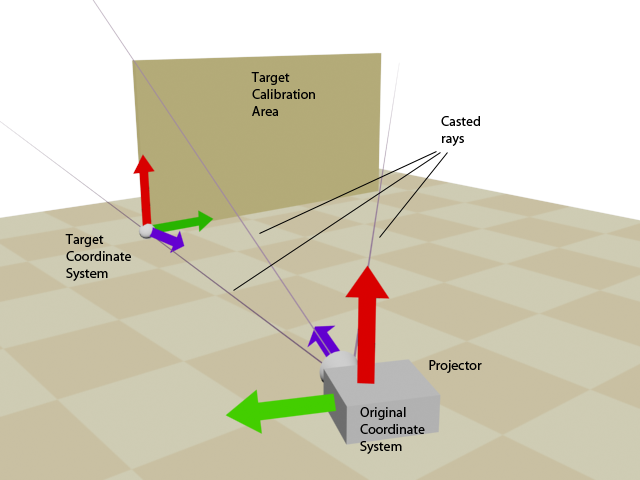
\includegraphics[width=0.7\textwidth]{./Cap2_videomapping/CalibrationSketch}
  \caption{Esquema de calibración.}
  \label{fig:CalibrationSketch}
\end{figure}
Usando las coordenadas en la pantalla de estos puntos y otros parámetros intrínsecos del proyector que son su resolución y el ángulo de proyección, es posible encontrar las coordenadas del punto con respecto al centro de proyección y por tanto la ecuación del rayo.
\[
a(t) = \vec{P} . t,	\mbox{ ecuación del rayo en dónde } \vec{P} \mbox{ es cualquier punto del rayo.}
\]
\[
\begin{cases}
P(X) = \frac{res_x}{2} - s_x \\
P(Y) = \frac{res_y}{2} - s_y \\
P(Z) = \frac{res_y}{2 \cdot \tan \frac{fov_y}{2}}
\end{cases}
\]
en donde $s_x$ y $s_y$ son las coordenadas del \emph{pixel}, $res_x$ y $res_y$ son la resolución horizontal y vertical del proyector y $fov_y$ es el ángulo de proyección vertical del proyector.

Aplicando esta ecuación a cada uno de los puntos a determinar se obtienen las ecuaciones paramétricas de los tres rayos. Vale aclarar que estos puntos $P$ son puntos de los rayos pero no necesariamente coinciden con los vértices de la superficie de calibración. Queda hallar las coordenadas de los vértices determinando el parámetro $t$ para cada ecuación. Para hallar este parámetro se resuelve un sistema de ecuaciones utilizando las tres ecuaciones de los rayos y las distancias conocidas entre estos puntos.
% Sistema de ecuaciones %
\[
\begin{cases}
\lVert{a(t_0) - b(t_1)} = j\rVert \\
\lVert{b(t_1) - c(t_2)} = k\rVert \\
\lVert{c(t_2) - a(t_0)} = l\rVert
\end{cases}
\]
siendo $a$, $b$ y $c$ los rayos y $j$, $k$ y $l$ las distancias entre las parejas de puntos.
La solución será entonces los parámetros $t_0$, $t_1$ y $t_2$ que satisfacen el sistema de ecuaciones no lineal.
Una aproximación a esta solución se puede obtener utilizando métodos numéricos, por ejemplo, el método \emph{trust-region-dogleg}\cite{TrustRegionDogleg}.
Una vez hallados los valores para $t_0$, $t_1$ y $t_2$, las coordenadas de los vértices de la superficie de calibración son $a(t_0)$, $b(t_1)$ y $c(t_2)$.
La base para el sistema de coordenadas con origen en el punto $P$ es:
\[
x' = \frac{b(t_1) - a(t_0)}{\lVert b(t_1) - a(t_0) \rVert},\quad y' = \frac{c(t_2) - a(t_0)}{\lVert c(t_2) - a(t_0)\rVert},\quad z' = -x' \times y'
\]
La ubicación del proyector en este nuevo sistema se obtiene proyectando cualquiera de los rayos en la nueva base de coordenadas.

\section{Tratamiento de malla}

Para la generacion mallas manejables por nuestra herramienta VMT se desarrollo un componente que se ejecuta separadamente y que recibe como entrada la nube de puntos a procesar. Como salida se generan mallas triangulares en el formato estandard OBJ.

%Rearmar la prosa de este primer párrafo%
Para la implementación de este módulo se utilizan los algoritmos descriptos en el estado del arte que incluye \emph{VcgLib} y que forman parte del procesamiento de malla propuesto. Para visualizar y evaluar los resultados esperados fue utilizada la aplicación de código abierto para la manipulación de mallas tridimensionales en diferentes formatos \emph{MeshLab} \cite{MeshLab}. Particularmente se utilizan los algoritmos de muestreo \emph{Poisson-disk} para reducir y normalizar los puntos de la malla inicial, \emph{normal extrapolation} para el cálculo de normales y reconstrucción de superficies de Poisson para la reconstrucción de la malla final.

Esta aplicación cuenta con una sencilla y única ventana que recibe los parametros para la configuración de los algoritmos que se ejecutan en cada uno de los pasos del procesamiento.

\begin{figure}[H]
  \centering
    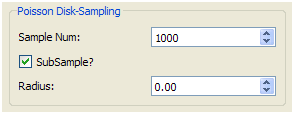
\includegraphics[width=0.5\textwidth]{./Cap2_videomapping/malla-poissongui.png}
  \caption{Configuración de parámetros del algoritmo \emph{Poisson-disk}}
  \label{fig:Mesh-PoissonGui}
\end{figure}

\begin{figure}[H]
  \centering
    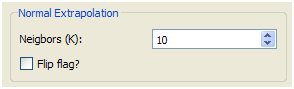
\includegraphics[width=0.5\textwidth]{./Cap2_videomapping/malla-normalextrapolation.png}
  \caption{Configuración de parámetros para reconstrucción de normales}
  \label{fig:Mesh-Extrapolation}
\end{figure}

\begin{figure}[H]
  \centering
    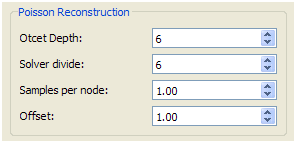
\includegraphics[width=0.5\textwidth]{./Cap2_videomapping/malla-poissonreconstruction.png}
  \caption{Configuración de parámetros para reconstruccion de malla de Poisson}
  \label{fig:Mesh-Normals}
\end{figure}


\subsection{Pruebas y resultados}

%Esta sección va dentro de lo que implementamos, recien aca salta que lo hicimos nosotros%

Para validar el correcto funcionamiento de esta técnica mediante los tres algoritmos descritos, fue utilizada una malla inicial de 5021 vértices y 9608 caras triangulares. Cabe destacar que si bien se ha mencionado que la malla de entrada debe ser simplemente una nube de puntos, se pueden utilizar mallas con caras, solo que estas serán ignoradas e incluso eliminadas de la malla de salida del primer paso del procesamiento (muestreo de \emph{Poisson-disk}).
Luego de experimentar con varios juegos de datos iniciales durante varias ejecuciones del procesamiento, se fijaron de manera personalizada para la malla de entrada algunos parámetros clave. Dado que la muestra inicial tiene alrededor de cinco mil puntos, fueron elegidas cinco mil muestras para el algoritmo de \emph{Poisson-disk}. Luego, para la extrapolación de normales se utilizan $K=15$ vecinos para la toma de decisiones locales de aproximación.
La aplicación de estos algoritmos resultó ser lo esperado en términos estructurales de cada malla procesada en cada uno de los pasos.
%Puede ir a trabajo futuro: No se llegó a procesar mallas de ambientes tridimensionales escaneados para luego ser mapeados con la herramienta.%

\begin{table}
\begin{center}
\begin{tabular}{|l||cc|} \hline
  Fase & Vértices & Caras \\
  Nube inicial & 5021 & 9608 \\
  Poisson-disk & 1776 & 0 \\
  Extrapolación Normales & 1776 & 0 \\
  Reconstrucción de Poisson & 1959 & 3910 \\ \hline %hay 1959 puntos en lugar de 1776, por que?%
\end{tabular}
\caption{Comparación de estructura de mallas de entrada y salida en cada fase}
\end{center}
\end{table}

\begin{figure}[H]
  \centering
    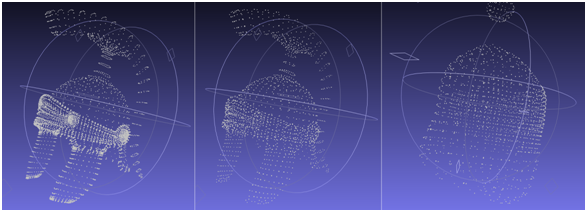
\includegraphics[width=0.8\textwidth]{./Cap2_videomapping/malla-nubepuntos.png}
  \caption{1) Nube de puntos inicial con 5021 vértices. 2) Resultado de muestreo \emph{Poisson-disk} con 1776 vértices. 3) Luego de extrapolar normales y reconstruir la malla con 1959 vértices y 3910 caras.}
  \label{fig:Mesh-Results}
\end{figure}
 
%Se observaron buenos tiempos computacionales de respuesta. Si bien la malla utilizada no es de un tamaño considerable, estamos hablando de algoritmos de orden relativamente alto.%

\clearpage\mbox{}
\chapter{Conclusiones y trabajos futuros}

En el marco de este proyecto se desarrolló la herramienta \emph{VMT} para la realización de espectáculos de \emph{video mapping} que implementa un enfoque novedoso, permitiendo la utilización de modelos tridimensionales para representar las superficies a proyectar y posibilitando la aplicación de efectos directamente sobre ellos. Cuenta con una interfaz de usuario interactiva en donde es posible visualizar los efectos en tiempo real a medida que se van diseñando.
Se lograron identificar etapas claramente diferenciadas en el proceso de creación de un espectáculo, lo cual fue muy útil para delinear requerimientos específicos para el desarrollo de \emph{VMT}. 

En las entrevistas que se mantuvieron con los \emph{VJs} éstos manifestaron un problema común que se da al utilizar más de un proyector cuyas proyecciones se solapan, causando deformaciones no deseadas en la visualización. \emph{VMT} mediante el soporte de múltiples proyectores evita este problema al tener control sobre qué objetos y efectos se muestran en cada proyector. Más en general, el manejo de múltiples proyectores distribuidos posibilita la creación de distintos esquemas de proyección soportando áreas amplias y disjuntas e incluso mapeos en 360 grados.

\subsubsection{Obtención automática de la geometría}

Se logró resolver parcialmente el problema de reconstrucción automática de la escena a mapear mediante la implementación de una aplicación que toma una nube de puntos ya capturada, la procesa y genera un objeto tridimensional para luego ser utilizado por \emph{VMT}.
Se trabajó en el estudio de las técnicas y componentes existentes para la reconstrucción tridimensional de la escena, principalmente mediante la utilización del método de luz estructurada en donde se experimentaron varios problemas, la mayoría de ellos en la etapa de calibración del sistema cámara-proyector. 

Se logró realizar exitosamente una prueba de concepto del método de escaneo de Kyle McDonald \emph{Three-Phase shift}.
Si bien este método logra obtener una representación tridimensional, tiene limitantes en cuanto a que las superficies a escanear deben ser continuas y sin cambios bruscos en la profundidad. Es por esta razón que no es aplicable para obtener geometrías correspondientes a escenas comúnmente utilizadas en espectáculos de \emph{video mapping}, ya que en general éstas contienen objetos que no cumplen estas características.

\begin{figure}[H]
  \centering
    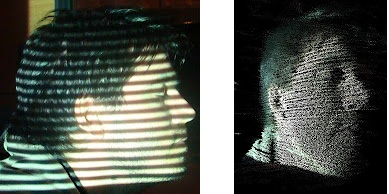
\includegraphics[width=0.7\textwidth]{./Cap7_conclusiones/Phase2.JPG}
  \caption[Imagen propia]{Izq: Patrón proyectado sobre sujeto de prueba. Der: Nube de puntos obtenida}
  \label{fig:cabeza}
\end{figure}

Se relevaron otros métodos de escaneo con luz estructurada que se adaptan mejor a un mayor rango de superficies, incluyendo las no soportadas por \emph{Three-Phase shift}, pero no se encontraron prototipos ya desarrollados para realizar pruebas de concepto y fue considerado fuera de los objetivos del proyecto.
Adicionalmente, durante el transcurso del proyecto surgió el dispositivo \emph{Kinect} para escanear objetos en tiempo real utilizando una implementación del método de luz estructurada. Con la liberación de su kit de desarrollo se incentivó su uso a desarrolladores de todo el mundo para una variedad de propósitos, lo que motivó a enfocar el alcance del proyecto en el procesamiento de nubes de puntos, independientemente de cómo estos puntos se obtienen, ya que \emph{Kinect} logra buenos resultados y es accesible en términos de costos.

Se implementó un prototipo de calibración tridimensional para obtener de forma automática la ubicación del proyector con respecto a una superficie.
Si bien este prototipo se pudo evaluar experimentalmente dando resultados que se aproximaban a lo esperado, necesitaba ajustes debido a las diferencias entre el funcionamiento de un proyector con el modelo ideal asumido. A su vez, el método de calibración se basa en parámetros intrínsecos del proyector como son su ángulo de enfoque el cuál debe ser medido experimentalmente, agregando errores a los cálculos.
En etapas posteriores del proyecto, al desarrollar la interfaz gráfica, se implementaron las transformaciones de cámaras virtuales mediante las cuales, si bien de forma manual, se puede lograr un ajuste más preciso.

\subsubsection{Espectáculos en vivo}

Se realizaron dos espectáculos en vivo con la herramienta \emph{VMT} en una versión alfa: el evento de cierre de Ingeniería de Muestra del año 2010\footnote{\url{http://www.fing.edu.uy/eventos/ingenieria_demuestra/2010/index.html}} de Facultad de Ingeniería de la Universidad de la República y un espectáculo durante la noche de fallos de fin de curso de Facultad de Arquitectura de la Universidad de la República.
\begin{figure}[H]
  \centering
    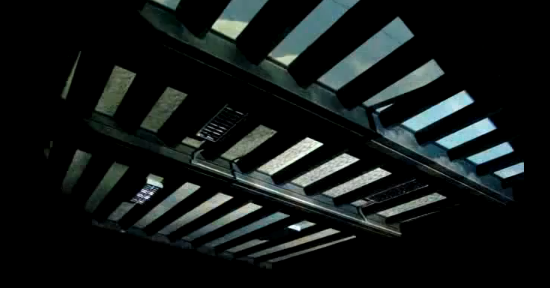
\includegraphics[width=0.7\textwidth]{./Cap7_conclusiones/ingMuestra1.png}
  \caption[Imagen propia]{Ingeniería de muestra 2010, \emph{quads} se iluminan al ritmo del audio.}
  \label{fig:ingMuestra1}
\end{figure}
\begin{figure}[H]
  \centering
    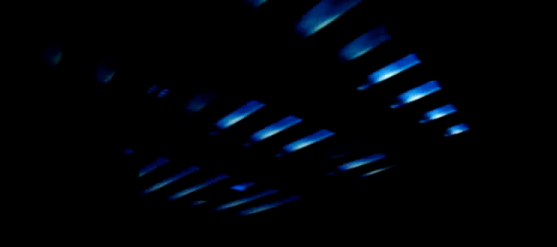
\includegraphics[width=0.7\textwidth]{./Cap7_conclusiones/ingMuestra2.png}
  \caption[Imagen propia]{Ingeniería de muestra 2010, videos en cada \emph{quad}.}
  \label{fig:ingMuestra2}
\end{figure}

\begin{figure}[H]
  \centering
    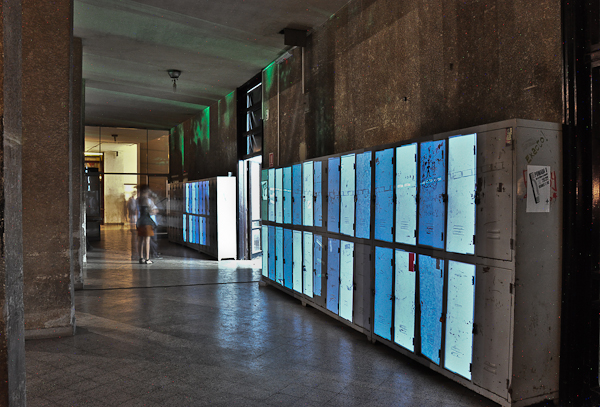
\includegraphics[width=0.7\textwidth]{./Cap7_conclusiones/Arqui1.jpg}
  \caption[http://www.farq.edu.uy/patio/conferencias-exposiciones-y-seminarios/noche-de-fallos-7.html]{Noche de fallos 2010, Fac. Arquitectura, casilleros iluminados.}
  \label{fig:Arquitectura1}
\end{figure}

\begin{figure}[H]
  \centering
    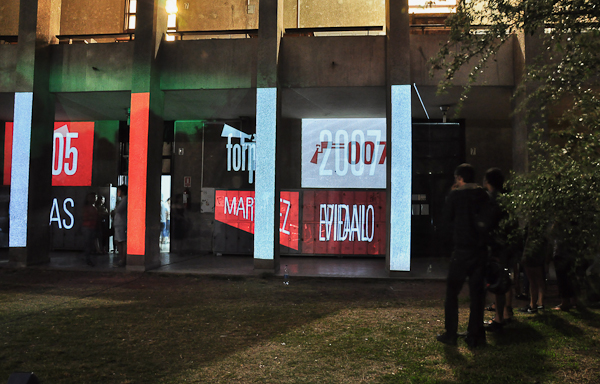
\includegraphics[width=0.7\textwidth]{./Cap7_conclusiones/Arqui2.jpg}
  \caption[http://www.farq.edu.uy/patio/conferencias-exposiciones-y-seminarios/noche-de-fallos-7.html]{Noche de fallos 2010, Fac. Arquitectura, casilleros y columnas iluminados.}
  \label{fig:Arquitectura2}
\end{figure}

\begin{figure}[H]
  \centering
    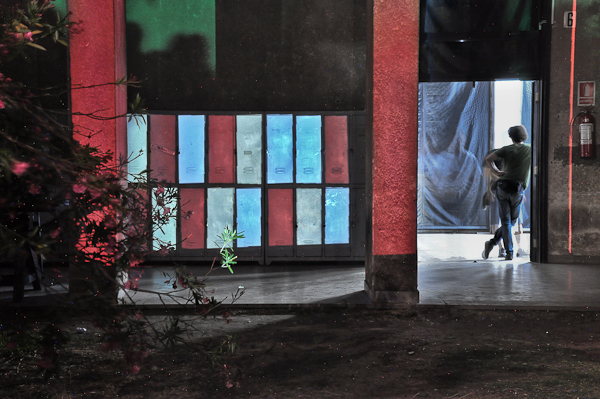
\includegraphics[width=0.7\textwidth]{./Cap7_conclusiones/Arqui3.jpg}
  \caption[http://www.farq.edu.uy/patio/conferencias-exposiciones-y-seminarios/noche-de-fallos-7.html]{Noche de fallos 2010, Fac. Arquitectura, casilleros y columnas cambiando de colores.}
  \label{fig:Arquitectura3}
\end{figure}

Durante la preparación y ejecución de los mismos se profundizó el conocimiento sobre lo necesario para llevar adelante un espectáculo de estas características, lo que ayudó a asentar las funcionalidades básicas que la aplicación debía cubrir. También se experimentó la importancia de la robustez y tolerancia a fallos que debe tener una aplicación que tiene como propósito la ejecución de espectáculos en vivo.

Desde el punto de vista funcional, se identificaron varios aspectos de la aplicación en las que se debía trabajar para mejorarlos, como ser el agregado de un mismo evento en varios momentos en la línea de tiempo, la agrupación de \emph{quads} para aplicarles el mismo efecto especificándolo una única vez y la ejecución del espectáculo a partir de un instante dado de la línea de tiempo. Todo lo anterior accesible mediante una interfaz gráfica de usuario que adopte criterios comúnmente utilizados en aplicaciones orientadas al diseño.

En las instancias iniciales del desarrollo de la aplicación, se había decidido distribuir los archivos contenedores de la definición del espectáculo en todos los nodos esclavo de \emph{VMT}, enviando desde el nodo maestro únicamente órdenes para ejecutar los efectos en el instante requerido.
Esto presentaba varios problemas, por ejemplo durante la edición del espectáculo, ante cualquier modificación en los \emph{quads} u objetos tridimensionales era necesario actualizar el archivo de definición en cada nodo y posteriormente reiniciarlo.
Debido a esta fuerte limitación se rediseñó la arquitectura y el protocolo de comunicación entre nodos maestro y esclavo, centralizando la definición del espectáculo en el nodo \emph{VMT} maestro y soportando la creación de todos los elementos mediante nuevos mensajes que fueron agregados a dicho protocolo.
Estos mensajes envían a cada nodo esclavo los objetos bidimensionales, tridimensionales, grupos de objetos, y efectos necesarios para la visualización del espectáculo en ese nodo en particular.
De estas experiencias también surgió el inconveniente de pérdida de mensajes durante la ejecución debido al uso de redes inalámbricas. Estas redes proveen facilidades para conectar nodos debido a que no requieren cableado pero tienen una alta tasa de colisiones. En el caso de \emph{VMT}, el uso de estas redes provocó que la pérdida de mensajes durante la ejecución ocasionara un desfasaje en la reproducción en los diferentes nodos esclavo. Por ello se decidió utilizar para el espectáculo de Facultad de Arquitectura una red cableada \emph{Ethernet} y se observaron mejoras notorias en cuanto a la calidad de la transmisión sin notar pérdida de mensajes.

\subsubsection{Trabajo futuro}

Durante el transcurso del proyecto en sus etapas de investigación del estado del arte y desarrollo de la aplicación \emph{VMT}, así como también producto de la experiencia obtenida en los dos espectáculos en vivo mencionados, se identificaron varias oportunidades de mejora de lo realizado y de esto se desprendieron nuevas líneas de trabajo a seguir.

Un aspecto en donde hay posibilidades de mejoras es la ampliación de las funcionalidades brindadas por la interfaz gráfica de usuario para permitir un uso más directo e intuitivo de la aplicación.
Esto se puede lograr permitiendo posicionar y editar elementos bidimensionales y tridimensionales directamente mediante acciones de ratón, sin dejar de soportar la opción de posicionamiento mediante el ingreso de coordenadas ya que esto permite un control más preciso.

\emph{VMT} permite únicamente utilizar \emph{quads} para representar figuras bidimensionales. Esto provoca que de necesitarse modelar figuras con más vértices para cubrir una superficie compleja sea necesario construirla utilizando más de un \emph{quad}. Una mejora posible sería permitir definir figuras bidimensionales con más de cuatro vértices para simplificar la definición en estos casos. Esto tiene la dificultad de que el mapeo de texturas no es directo para figuras con más de cuatro vértices por lo que la aplicación debería proveer un mecanismo para definir las coordenadas de mapeo para cada vértice. De todas formas, esta funcionalidad se puede cubrir mediante el uso de objetos \emph{3DS} que ya incorporen las coordenadas de mapeo en los vértices.

Para el manejo de objetos tridimensionales, \emph{VMT} depende de herramientas externas que permitan el manejo de archivos \emph{3DS}. En particular, las tareas que serían deseables incluir en \emph{VMT} son las de edición de vértices y caras de mallas tridimensionales y asignación de materiales a grupos de caras.

Actualmente \emph{VMT} no dispone de una interfaz visual que asista a la sincronización de la ejecución de los efectos visuales con el audio que acompaña el espectáculo.
Una forma en que esto podría realizarse es desplegando una visualización de la onda de audio, para tener una idea de en qué instantes se provocan cambios importantes en el sonido y asignar efectos directamente en los instantes visualizados.

Por último, debido al amplio estudio en métodos de obtención automática de geometría tridimensional y a la más reciente liberación del kit de desarrollo de \emph{Kinect} sería de interés integrar la captura de geometría con \emph{VMT} para permitir un uso más dinámico de la aplicación, de esta forma completando el ciclo de trabajo para la construcción de un espectáculo de \emph{video mapping}.


\appendix

\chapter{Aportes}
\label{chapter:aportes}
A continuación se presentan los resultados de una serie de entrevistas realizadas a \emph{VJs} e ingenieros contactados a partir de la investigación del estado del arte del \emph{video mapping}. Se les consultó sobre sus trabajos realizados y las técnicas y herramientas que utilizaron para su producción.
Fueron introducidos brevemente al proyecto para recibir comentarios y conocer sus expectativas en cuanto a herramientas que puedan asistirlos en la resolución o simplificación de problemas con los que se encuentran actualmente al momento de realizar espectáculos de \emph{video mapping}.

\section{Marcelo Vidal (VJ Chindogu)}
Marcelo Vidal\cite{Chindogu} es un \emph{VJ} local referente del \emph{video mapping} en nuestro medio y quien ha desarrollado varios de los espectáculos más importantes y de gran repercusión.
Nos comenta que para sus espectáculos trabaja principalmente con modelos en dos dimensiones, por lo que la fase inicial de su trabajo se basa en transformar la fachada o superficie a mapear en un modelo bidimensional.
Para este propósito su forma de trabajo consiste en fijar la posición y orientación del proyector en el lugar desde donde se realizará la proyección, para luego capturar las formas y construir el modelo bidimensional.

Una vez modelada la escena, se realiza todo el trabajo creativo y de diseño visual del espectáculo, para lo que utiliza \emph{AfterEffects}, \emph{Photoshop} y \emph{3D Studio}. Luego, al momento de la proyección, posiciona nuevamente el proyector en el lugar original y realiza los ajustes previos. Entre estos ajustes se encuentra la calibración y posicionamiento del proyector en donde fue resaltada la dificultad existente para mover los proyectores que se utilizan en espectáculos de gran porte, los que pueden llegar a pesar hasta 200 kilogramos, lo que dificulta realizar movimientos milimétricos para ajustes finos. Por esto último considera importante la disposición de herramientas de ajuste o calibración del modelo de software sobre la superficie. Destacó que utiliza exactamente el mismo proyector tanto para la obtención de la geometría como para la posterior ejecución del espectáculo, lo cual según su experiencia reduce el trabajo posterior de calibración.

En cuanto al mapeo, fue destacado como muy importante poder tener la posibilidad de modificar en tiempo real el espectáculo. En referencia al tratamiento de las deformaciones que se producen al proyectar sobre una superficie irregular, comentó que maneja diferentes estrategias. Puede tanto utilizar la deformación dada por la superficie junto con deformaciones de la imagen o video a proyectar para lograr un efecto en conjunto, como también intentar modificar el video o imagen para minimizar los efectos dados por la superficie irregular. Comenta que esta última opción es la menos interesante en el ámbito artístico de los \emph{VJs}. Las herramientas que utiliza para la realización de sus espectáculos son \emph{QuickTime}, \emph{Module8}, \emph{VDMX} y \emph{Resolume PC}.

\section{Martin Borini (\emph{VJ Ailaviu})}
La principal inquietud que nos transmitió Martín Borini\cite{Ailaviu} fue en relación al manejo de información tridimensional durante el proceso de producción de un espectáculo y así poder conocer las deformaciones que se darán en la superficie donde se proyectará. También se muestra preocupado por el problema de la correspondencia entre el modelo tridimensional y la superficie, lo que lo lleva a estar interesado en la posibilidad de la calibración de un modelo de ese estilo.
En sus trabajos realizados sobre fachadas ha tomado fotos a nivel desde el mismo lugar donde se coloca el proyector. Según su experiencia esto produce mejores resultados que trabajar sobre planos o medidas tomadas por él. Otro punto en el cual expresó interés fue en casos en los que se utilizan más de un proyector, en donde surge el problema de las costuras o uniones de las imágenes proyectadas por los diferentes proyectores.

\section{Viktor Vicsek}
Viktor Vicsek\cite{Viktorvicsek} es un \emph{VJ} de nivel internacional y se ha establecido contacto con él luego de observar los espectáculos de más relevancia y popularidad referenciados en sitios relacionados al tema. Comenta que ha implementado sus propios módulos de software para asistirle en la producción. También ha realizado una mejora a la técnica de calibración automática de proyectores de Johnny Lee\footnote{http://johnnylee.net/projects/thesis} utilizando cámaras y visión por computadora en lugar de sensores de luz, lo que le ha resultado particularmente útil al trabajar con grandes superficies o fachadas de edificios. También ha implementado su propia línea de tiempo de videos utilizando \emph{Adobe Air}. Para la realización de los mapeos y distorsiones de imágenes y videos utiliza la herramienta de programación visual \emph{VVVV}.

Su proceso de producción consta en tomar fotografías y obtener los planos arquitectónicos de la escena en cuestión y la creación del modelo, según sus necesidades, con herramientas de modelado como \emph{3D Studio}. Posteriormente realiza el mapeo de texturas de imagen o video aplicando efectos que utilizan \emph{shaders} sobre el modelo mediante la utilización de \emph{VVVV}.
\clearpage\mbox{}
\chapter{Relevamiento de aplicaciones de \emph{video mapping}}
\label{chapter:aplicaciones}
\section{\emph{Modul8}}
\emph{Modul8} \cite{Module8} es una herramienta profesional para realizar espectáculos de proyección de video en vivo diseñada por \emph{VJs} y se encuentra disponible exclusivamente para plataforma \emph{Mac OS X} mediante licenciamiento propietario.%se dice licenciamiento propietario?%

\begin{figure}[H]
  \centering
    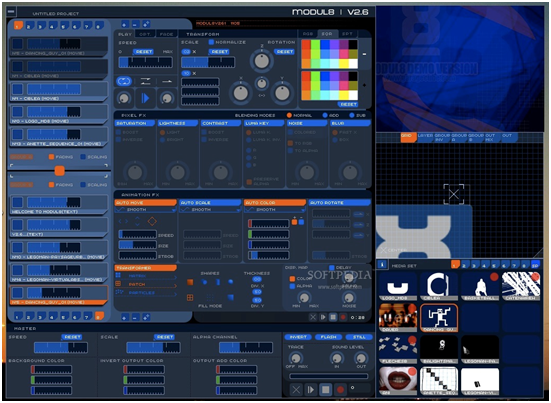
\includegraphics[width=0.6\textwidth]{./Apendices/Cap3_aplicaciones/apps-modul8.png}
  \caption{Pantalla principal de \emph{Modul8}}%referenciar%
  \label{fig:Apps-Module8}
\end{figure}

La interfaz de usuario está pensada para los espectáculos en vivo, para lo que cuenta con cuatro paneles con un fin específico: un panel principal donde crear y editar las composiciones de video, sonido y efectos; un panel multimedia para administrar los archivos de medios (videos, imágenes, pistas de audio, etc.); un panel de previsualización donde se puede ir observando la ejecución de una parte de la composición del espectáculo; y por último el panel de salida, donde se observa la composición final que será proyectada. Todas las funcionalidades provistas pueden ser asignadas a eventos \emph{MIDI}, por lo que es posible utilizar cualquier dispositivo que los genere para controlar enteramente la aplicación.
\emph{Modul8} maneja hasta siete salidas simultáneas de proyección y una más para la interfaz de usuario. Para hacer uso de esta funcionalidad es necesario contar con una tarjeta de video que dé soporte a la salida múltiple. Esto activa el modo de salida avanzado donde se puede escoger entre varias alternativas para la selección de la composición o porción de la misma a ser emitida en cada una de las salidas disponibles. \emph{Modul8} maneja el concepto de capa, con un máximo de diez, las cuales pueden contener sus propios medios, efectos y configuraciones.
Si bien no hay un manejo tridimensional de la escena, la aplicación provee algunas transformaciones a aplicar a los medios para ajustarlos a la representación bidimensional de los objetos de la escena o incluso a objetos tridimensionales autogenerados que aparecerán en la misma.
La arquitectura de la herramienta permite su extensión mediante la programación de módulos o efectos en el lenguaje \emph{Python}\footnote{www.python.org}.
En relación al rendimiento, se hace un uso intensivo de la unidad de procesamiento gráfica o \emph{GPU}$^\dagger$ para todo lo que es dibujado, composición y transformaciones de gráficos.
%Agregar madmapper y hablar de la integración con modul8%

\section{\emph{VDMX}}
\emph{VDMX} \cite{VDMX} es una aplicación para el procesamiento multimedia en tiempo real, disponible exclusivamente para plataforma \emph{Mac OS X} mediante licenciamiento propietario. Su arquitectura modular la hace altamente personalizable.

\begin{figure}[H]
  \centering
    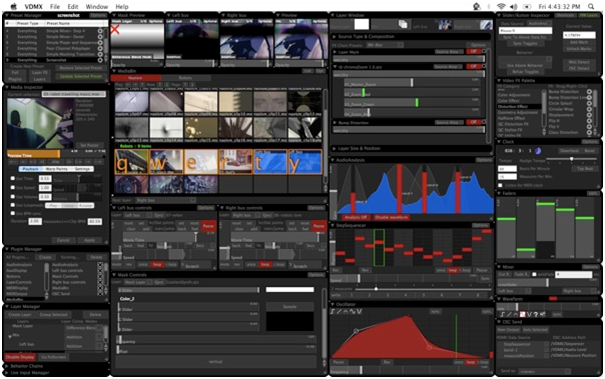
\includegraphics[width=0.6\textwidth]{./Apendices/Cap3_aplicaciones/apps-vdmx.png}
  \caption{Ejemplo de consola personalizable avanzada realizada en VDMX} %referenciar%
  \label{fig:Apps-VDMX}
\end{figure}

%No se puede empezar un párrafo diciendo Para ello.., se habla de herramientas como QuartzComposer sin mencionar que son%
Para ello provee funcionalidad básica mediante lo que la aplicación denomina \emph{inspectores}. El \emph{inspector} del grupo de trabajo expone todo lo que esta sucediendo en \emph{VDMX} a bajo nivel, por ejemplo, los archivos multimedia, las entradas de video configuradas, las capas, los \emph{plugins} existentes, etc. Luego, el \emph{inspector} de interfaz de usuario permite ver y editar las propiedades de cada control que se selecciona en la interfaz. Adicionalmente, permite crear interfaces propias a partir de controles básicos como deslizadores, botones, ventanas emergentes, etc, lo que permite a los \emph{VJs} tener toda la información que crea relevante a disposición en el momento de la representación en vivo.
La aplicación permite asociar eventos de entrada \emph{MIDI}, \emph{OSC} o de teclado a cualquier control de la interfaz de usuario, así como también generar eventos \emph{MIDI} u \emph{OSC} para ser consumidos por otras aplicaciones.
Las capas contienen una única fuente de medios, la que puede ser de tipo video, composición de \emph{QuartzComposer}\footnote{quartzcomposer.com} o imagen, y adicionalmente se define una cadena de efectos a ser aplicados a la fuente de la capa. La ejecución de la secuencia de efectos puede ser configurada mediante cualquiera de los mecanismos de eventos mencionados anteriormente así como por tiempo. No hay un máximo establecido en el número de capas que se pueden crear en \emph{VDMX}, y es posible agruparlas para darle un manejo diferenciado o aplicar efectos a todas a la vez.
Se cuenta con tres modos de salida de video: ventana, pantalla completa y avanzado. En el modo avanzado se permite definir dispositivos de salida, sin un límite predeterminado, y asociarlos a las capas o dispositivos de entrada que se desee.

%Agregar Syphon y Resolume%

\section{\emph{VVVV}}
\emph{VVVV} \cite{VVVV} es una herramienta de programación de propósito general que provee un entorno híbrido de programación gráfica y textual. Es de uso gratuito para propósitos no comerciales y se encuentra disponible únicamente para plataformas \emph{Windows}.

\begin{figure}[H]
  \centering
    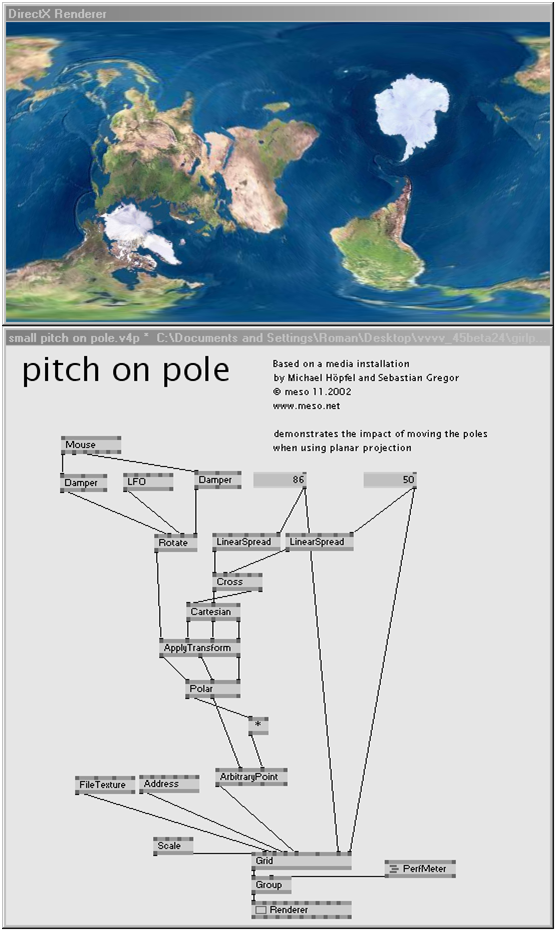
\includegraphics[width=0.5\textwidth]{./Apendices/Cap3_aplicaciones/apps-vvvv.png}
  \caption{Entorno de programación de \emph{VVVV} y salida de video correspondiente}
  \label{fig:Apps-VVVV}
\end{figure}

Para la construcción de un programa se utilizan nodos que representan operaciones o funciones individuales que pueden tomar una entrada, procesarla, y entregar datos a la salida. Las conexiones entre nodos se llaman \emph{links} y es cómo se modela el flujo de información entre nodos.
Existen varios tipos de nodos para diferentes propósitos. A modo de ejemplo, el nodo utilizado para desplegar la salida visual del programa es del tipo \emph{Renderer}, para el agregado de cuadrantes se utiliza el nodo \emph{Quad}, para el manejo de transformaciones el nodo \emph{Transform} y para redimensionar a escala el nodo \emph{Scale}. También hay nodos para cargar objetos tridimensionales, manejar texturas, vectores, temporizadores, etc.
A diferencia de otros lenguajes de programación, que cuentan con diferentes modos para construir y ejecutar los programas, \emph{VVVV} todo el tiempo trabaja en un solo modo, el modo de ejecución. En él, constantemente se están ejecutando cálculos y dibujando gráficos mientras se está generando o editando un programa.
Para dar soporte multiproyector, \emph{VVVV} implementa una arquitectura cliente-servidor, la que permite contar con cualquier cantidad de motores tridimensionales (clientes) manejados desde una instancia de \emph{VVVV} central (servidor). Toda la configuración y ejecución de un espectáculo distribuído se implementa en un módulo llamado \emph{boygrouping}\footnote{http://vvvv.org/documentation/boygrouping-basics}.
\emph{VVVV} provee soporte para varios protocolos de entrada y salida como \emph{TCP}, \emph{UDP}, \emph{MIDI} y \emph{OSC} entre otros, y gracias a aportes de la comunidad de programadores \emph{VVVV} es posible también interactuar con dispositivos como \emph{Wii}, \emph{PSP} y \emph{Kinect}. Existen nodos que proveen funcionalidad avanzada como ser soporte para animación y líneas de tiempo, detección y seguimiento de objetos en tiempo real utilizando técnicas como \emph{ARToolkit} y \emph{OpenCV}, emisión de flujos de video, reproducción y mezcla de archivos de audio, simulación de movimiento, colisiones y efectos físicos en general.
El motor gráfico tridimensional de \emph{VVVV} está basado en \emph{Direct3D}, lo que permite hacer un uso intensivo de las placas gráficas modernas para el dibujado de gráficos de alto rendimiento.
\emph{VVVV} ofrece la posibilidad de crear nodos personalizados a través de una interfaz \emph{COM} para la implementación de \emph{plugins}, lo que ofrece alternativas en cuanto a la implementación, pudiéndose utilizar \emph{C\#}, \emph{Delphi} o \emph{C++}.

\section{\emph{VPT - Video Projection Tool}}
\emph{VPT} \cite{VPT} es una herramienta para la realización de proyecciones en tiempo real. Es una aplicación de uso y distribución gratuita. Se encuentra disponible para plataformas \emph{Windows} y \emph{MacOS}.

\begin{figure}[H]
  \centering
    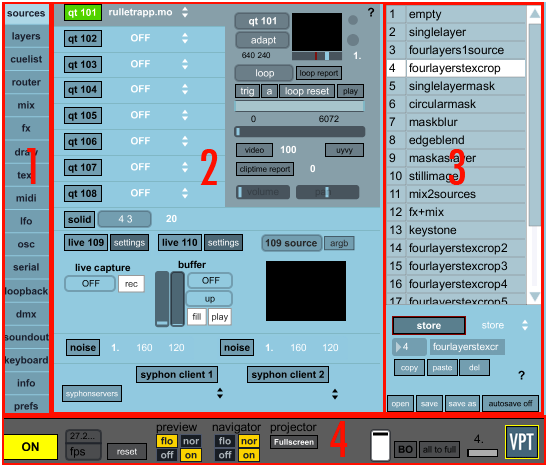
\includegraphics[width=0.65\textwidth]{./Apendices/Cap3_aplicaciones/apps-vpt.png}
  \caption{Pantalla principal de \emph{VPT}}%ref%
  \label{fig:Apps-VPT}
\end{figure}

La interfaz gráfica es amplia y permite el acceso a variadas funcionalidades. Dispone de una barra de herramientas con cada una de las secciones, las que se muestran en detalle en el panel principal de la aplicación. Siempre disponible a la derecha, están las configuraciones establecidas y predefinidas. La barra sobre el borde inferior de la pantalla es desde donde se controlan las salidas de video, la previsualización y las opciones de navegación.
En cuanto a los posibles orígenes de medios, se puede contar con hasta ocho videos de \emph{Quicktime}, dos entradas en vivo, las que pueden ser asociadas a cualquier dispositivo de video soportado en el sistema, y una entrada de dibujado en la que es posible crear máscaras personalizadas para objetos sobre los cuales se proyectará.
Hay una cantidad máxima de 32 capas que se pueden utilizar simultáneamente en un espectáculo. Cada una está superpuesta sobre la siguiente, y puede ser escalada, posicionada, rotada, distorsionada y enmascarada de manera independiente. Maneja el concepto de capa activa para la edición y dibujado en la ventana de salida y cuenta con una secuencia de eventos a partir de efectos predefinidos almacenados y configurados previamente en el sistema. Para la definición de efectos se cuenta con tipos predefinidos y una nomenclatura para agregarlos a la lista, por ejemplo ``F 15 16 5.00'' representa una transición del efecto 15 al 16 con duración 5 segundos, ``C 5'' ejecuta el efecto número cinco, ``L 3'' genera un bucle y vuelve al tercer lugar de la lista de eventos, ``D 2'' genera una demora de dos segundos y continúa con el siguiente evento, etc.

\begin{figure}[H]
  \centering
    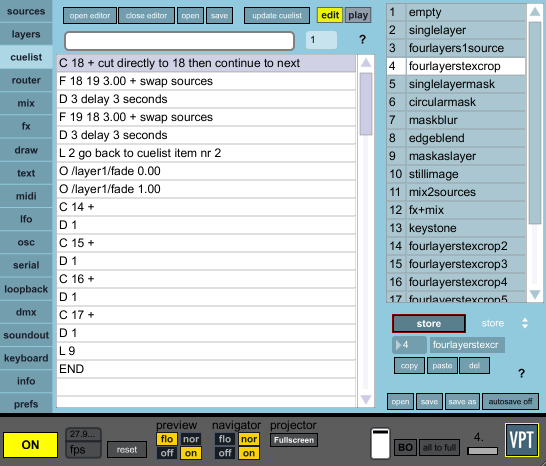
\includegraphics[width=0.65\textwidth]{./Apendices/Cap3_aplicaciones/apps-vpt-cuelist.png}
  \caption{Efectos y secuencia de eventos de un espectaculo realizado en VPT}%ref%
  \label{fig:Apps-VPTCuelist}
\end{figure}

Dentro del modo de edición es posible agregar o eliminar elementos a la lista sin que estos sean reflejados en la salida de video, mientras que en modo de reproducción se está recorriendo la lista de efectos constantemente, generando la salida correspondiente.
Dependiendo de la tarjeta de sonido con la que se cuente, es posible direccionar las entradas de video en hasta ocho canales de salida de audio. El módulo de mezclado permite combinar dos orígenes cualesquiera utilizando diferentes modos. También es posible controlar la aplicación o enviar directamente indicaciones a las capas, orígenes de medios, mezclador, etc, utilizando \emph{OSC}, \emph{MIDI} o vía puerto serial con dispositivos como \emph{arduino}\footnote{http://www.arduino.cc}.
Para simular proyecciones tridimensionales se cuenta con la posibilidad de subdividir las texturas con grillas y aplicar así distorsiones a distintos sectores de la misma.
%Ver aquí un ejemplo de mallas combinado con el uso de MacOS Syphon Recorder (Syphon MacOS Plugin http://syphon.v002.info/). (http://hcgilje.wordpress.com/2011/05/26/vpt-5-5-preview/)

\clearpage\mbox{}
\chapter{Método de triangulación}

Mediante este método se determinan las coordenadas $(x,y,z)$ de un punto utilizando la posición bidimensional dada por las perspectivas de dos proyecciones de las que se conocen los centros de perspectiva y planos de proyección\cite{PresUnivYonsei}.

Escena con dos dimensiones:

\begin{figure}[H]
  \centering
    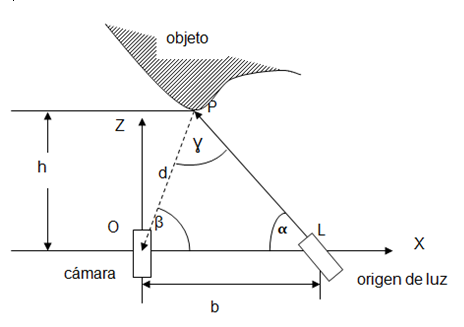
\includegraphics[width=0.65\textwidth]{./Cap2_videomapping/triangulacion.PNG}
  \caption[Imagen propia.]{Propiedades trigonométricas para escena bidimensional.}
  \label{fig:Triangulacion}
\end{figure}

Este método tiene como objetivo calcular la distancia $d$ de la cámara al punto $P$ a partir de los ángulos $\alpha$, $\beta$ y la distancia $b$ entre el proyector y la cámara.
El ángulo $\alpha$ y la distancia $b$ son dados por la configuración de la escena.
El ángulo $\beta$ está dado por la geometría de la proyección.

\[
\left.
\begin{array}{l}
\frac{d}{\sin (\alpha)} = \frac{b}{\sin (\gamma)} 	\\
\gamma = \pi - (\alpha + \beta)						\\
\sin (\pi - \gamma) = \sin (\gamma)
\end{array}
\right \rbrace
\frac{d}{\sin(\alpha)} = \frac{b}{\sin(\pi - \gamma)} = \frac{b}{\sin(\alpha + \beta)} \Rightarrow d = b . \frac{\sin(\alpha)}{\sin(\alpha + \beta)}
\]

Las coordenadas cartesianas quedan determinadas por:
\[
X_0 = d. \cos (\beta)
\]
\[
Z_0 = d. \sin (\beta) = h
\]

Escena con tres dimensiones:

\begin{figure}[H]
  \centering
    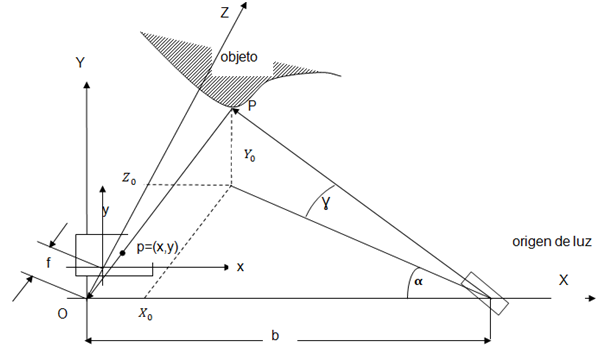
\includegraphics[width=0.65\textwidth]{./Cap2_videomapping/triangulacion-2.PNG}
  \caption[Imagen propia.]{Propiedades trigonométricas para escena tridimensional.}
  \label{fig:Triangulacion2}
\end{figure}

Se asume $Z = f$ siendo $f$ el plano en el cuál se proyecta el punto $P(X_0, Y_0, Z_0)$, obteniendo como resultado de la proyección el punto $p(x,y)$.
El centro óptico del proyector está situado en el eje $X$.
Se considera realizada una pre-calibración en la cual se define:
\[
P = (x,y), \quad \frac{X_0}{x} = \frac{Z_0}{f} = \frac{Y_0}{y} = k \to (k * x,k * y,k * f)
\]
Por trigonometría:
\[
\tan (\alpha) = \frac{Z_0}{(b - X_0)} \Rightarrow Z_0 = \tan (\alpha) (b - X_0) \quad 
\]
\[
k * f = \tan (\alpha)(b - k * x)
\]
\[
k (f + x * \tan (\alpha)) = b * \tan (\alpha)
\]
\[
k = \frac	{b * \tan (\alpha)}{f + x * \tan (\alpha)}
\]
\[
X_0 = \frac{x * b * \tan (\alpha)}{f + x * \tan (\alpha)}, \quad Y_0 = \frac{y * b * \tan (\alpha)}{f + x * \tan (\alpha)},\quad Z_0 = \frac{f * b * \tan (\alpha)}{f + x * \tan (\alpha)}
\]
\clearpage\mbox{}
\chapter{Modelo de cámara}

\section{Modelo \emph{pinhole}}

Una cámara, por medio de una proyección central, establece una correspondencia entre puntos del espacio con puntos bidimensionales en su plano imagen. En particular se estudia el modelo de cámara \emph{pinhole} \cite{LibroCompGrafica3}.

Se considera el centro de proyección $C$, también centro óptico de la cámara, como el origen de un sistema de coordenadas euclideano, y $Z = f$ el plano de la imagen o plano focal.

\begin{figure}[H]
  \centering
    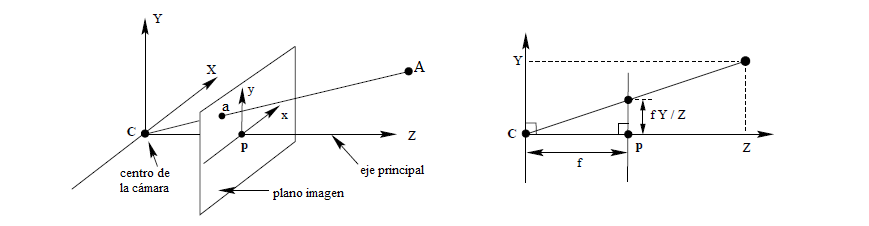
\includegraphics[width=0.8\textwidth]{./Cap2_videomapping/pinhole.png}
  \caption[Multiple View Geometry in Computer Vision, Fig. 6.1]{Geometría de cámara \emph{pinhole}. $C$ es centro de la cámara y $p$ el punto principal}
  \label{fig:Calib-Pinhole}
\end{figure}

Un punto en el espacio $A=(A_X, A_Y, A_Z)^T$ se corresponde con el punto $a$ en el plano imagen, dado por la intersección del rayo que pasa por el centro de cámara y el punto $A$ con el plano imagen. El punto $A$ se corresponde con $(\frac{fA_X}{A_Z}, \frac{fA_Y}{A_Z}, f)^T$ en el plano imagen considerando que el centro de coordenadas del plano coincide con el punto principal $P$.

Considerando la representación de los puntos como vectores homogéneos se expresa la proyección central como una correspondencia lineal entre las coordenadas homogéneas.

\[
\begin{pmatrix}
A_X \\ A_Y \\ A_Z \\ 1
\end{pmatrix}
\to
\begin{pmatrix}
fA_X \\ fA_Y \\ A_Z
\end{pmatrix}
=
\begin{pmatrix}
f & 0 & 0 & 0 \\
0 & f & 0 & 0 \\
0 & 0 & 1 & 0 \\
\end{pmatrix}
\begin{pmatrix}
A_X \\ A_Y \\ A_Z \\ 1
\end{pmatrix}
\]

Dado $A_h = (A_X,A_Y,A_Z,1)^T$ y la proyección $a$ sobre el plano imagen, la correspondencia utilizando el método pinhole es:
$a=PA_h$

Siendo
\[
P = 
\begin{pmatrix}
f & 0 & 0 & 0 \\
0 & f & 0 & 0 \\
0 & 0 & 1 & 0 \\
\end{pmatrix}
\]

\section{Geometría epipolar}
La geometría epipolar\cite{LibroCompGrafica3} es la geometría proyectiva intrínseca entre dos puntos de vista. Es dada por la intersección de los planos imagen de cada cámara con el plano epipolar. Este plano es el definido por el punto a representar $X$ y los dos centros de las cámaras $C$ y $C'$.

\begin{figure}[H]
  \centering
    \includegraphics[width=0.7\textwidth]{./Cap2_videomapping/epipolar.PNG}
  \caption[Multiple View Geometry in Computer Vision, Fig. 9.1]{$C$ y $C'$ centros de las cámaras.}
  \label{fig:Epipolar}
\end{figure}
La matriz fundamental $F$ es la representación algebraica de la geometría epipolar.
Dado un par de imágenes, como se muestra en la figura para cada punto $x$ en una imagen existe una línea epipolar correspondiente $l'$ en la otra imagen. Cualquier punto $x'$ en la segunda imagen que corresponde al punto $x$, debe pertenecer a la línea epipolar $l'$.
La línea epipolar $l'$ es la proyección en la segunda imagen del rayo que parte del punto $x$ y llega al centro $C$ de la primer cámara. Se establece por tanto un mapeo de un punto en una imagen con la línea epipolar en la otra imagen.
\[  x \to l'
\]
 
El mapeo de puntos a líneas es representado por $F$ la matriz fundamental.

\begin{figure}[H]
  \centering
    \includegraphics[width=0.7\textwidth]{./Cap2_videomapping/epipolar2.PNG}
  \caption[Multiple View Geometry in Computer Vision, Fig. 9.5]{Matriz fundamental $F$.}
  \label{fig:Epipolar2}
\end{figure}
Dado $x$ en una imagen se corresponde con el punto $x'$ en la segunda imagen vía una trasferencia establecida por la intersección del plano $\pi$ con los planos imagen de cada cámara.
La línea epipolar que contiene $x'$ se obtiene uniendo $x'$ con el epipolo $e'$, esto es:
\[ x' = H_{\pi} * x \]    siendo  $H_{\pi}$ una homografía 2D que establece la correspondencia entre cada $x_i$ de la primer imagen a $x'_i$ en la segunda imagen.
\[ l' = e' * x' = e' * H_{\pi} * x = F * x  \]
\[ F = e' * H_{\pi}  \mbox{es la matriz fundamental}  \]
\clearpage\mbox{}
\newpage
\bibliographystyle{alpha}
\addcontentsline{toc}{chapter}{Bibliografía}
\bibliography{./bibliografia}

\newpage
\printgloss{./glosario}
\newpage
\listoffigures

\end{document} 
